\chapter{Autonomous Driving and HD Maps}
The goal of this Chapter is to provide an overview of High Definition (HD) maps and their importance in the field of Autonomous Driving. It examines the state-of-the-art localization techniques on HD maps to establish the context for introducing MapAlign, the project developed in this thesis.

\section{Introduction to Autonomous Driving (AD)}
The concept of \textit{autonomous driving} has evolved from a theoretical idea to a rapidly advancing field with deep technological, societal, and legal implications. Autonomous vehicles (AVs) hold the potential to revolutionize transportation by improving safety, reducing congestion, and enhancing mobility \cite{9695620}. The technological backbone of this transformation involves advanced sensors, machine learning and deep learning algorithms, vehicle-to-everything (V2X) communication, and real-time decision-making algorithms.

At the core of understanding the complexity and potential of autonomous vehicles lies the classification system developed by the Society of Automotive Engineers (SAE)\footnote{The Society of Automotive Engineers (SAE) is a global organization that established a standardized framework for defining and categorizing levels of driving automation. This framework is intended to clarify the roles of human drivers and automated systems, ensuring consistent standards for safety and functionality across various levels of automation.} \cite{SAE_J3016_202104}, which defines the various stages of vehicle automation.

The SAE International established a six-tier classification system in 2014, which was refined in subsequent years, to standardize the levels of driving automation across the industry. The levels range from Level 0, where no automation exists, to Level 5, representing full automation. Each level represents a step toward the ultimate goal of a fully autonomous vehicle, and these levels are essential in understanding the current and future development of AV technology \cite{9881892}.

Figure~\ref{fig:sae_levels} illustrates these levels, detailing the progression of driving automation and the key distinctions between each stage.
\begin{figure}[H]
    \centering
    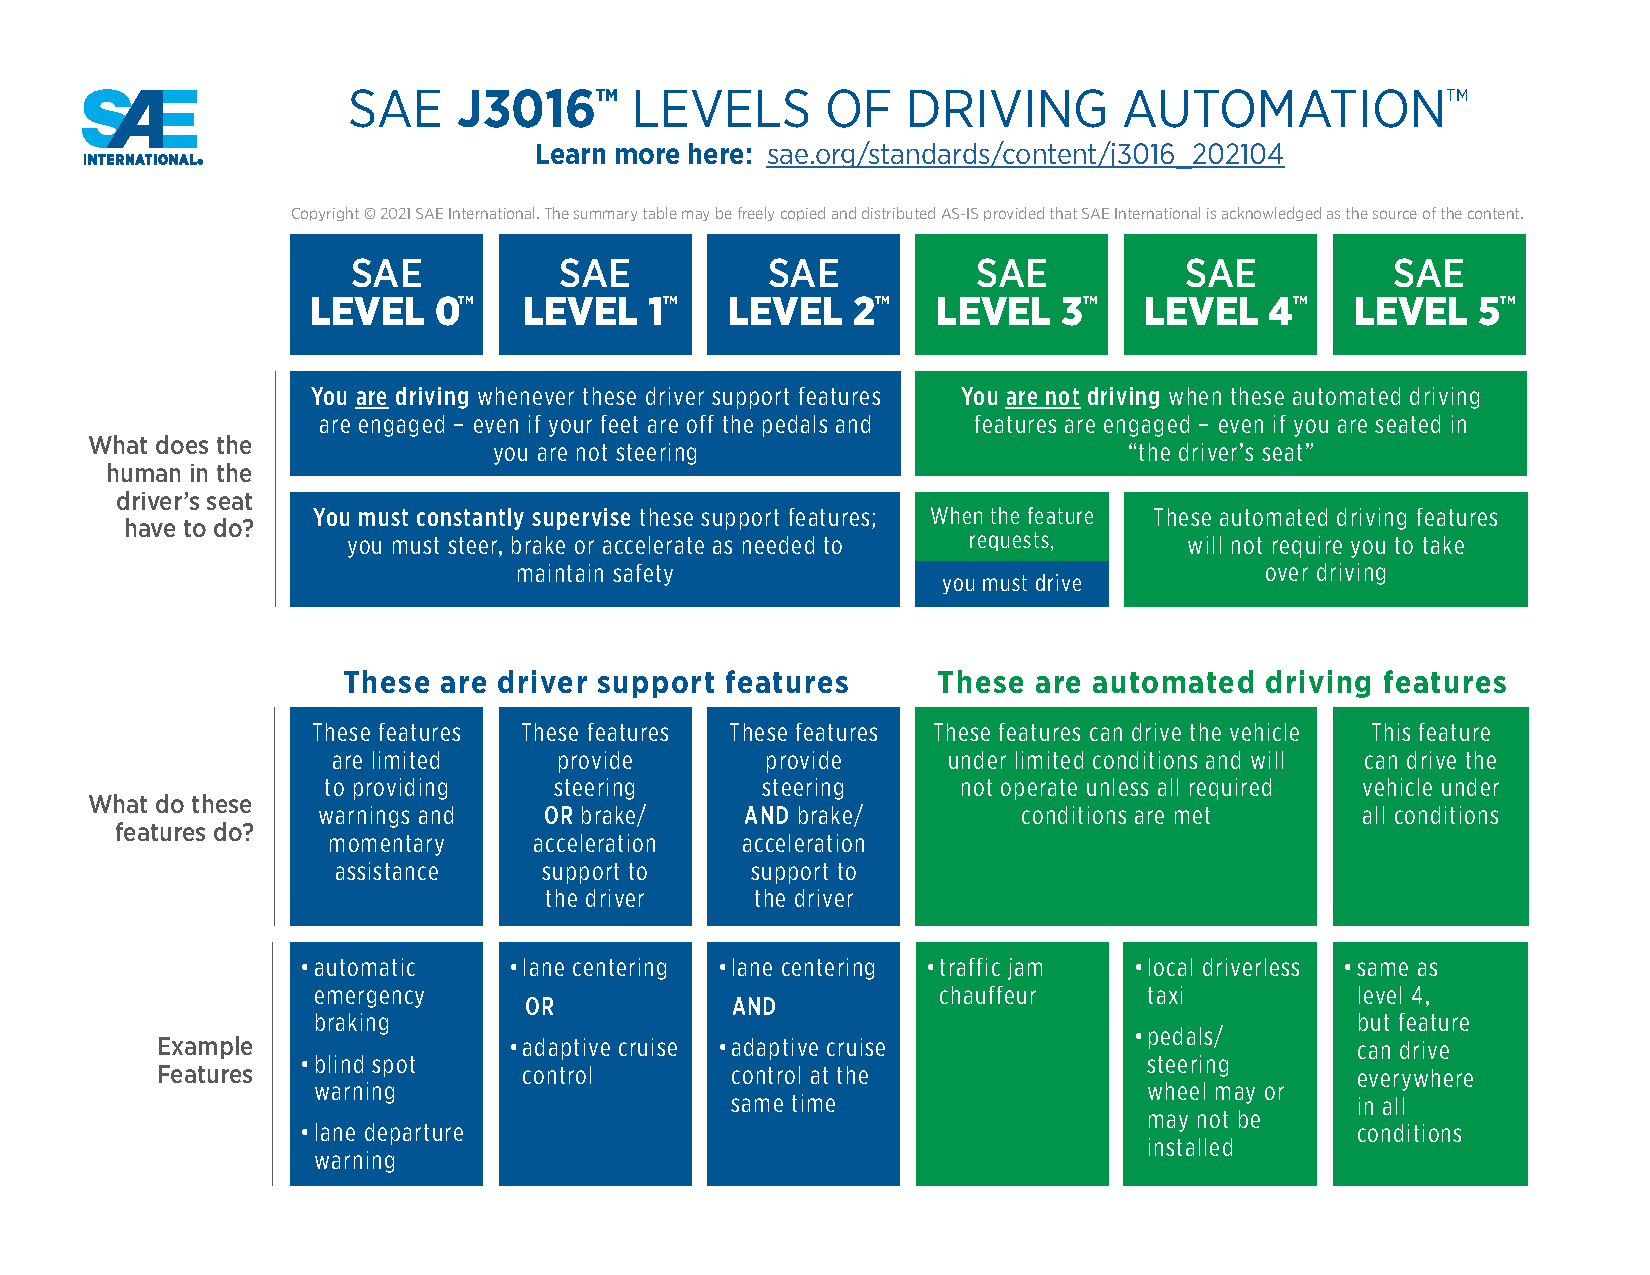
\includegraphics[width=1\linewidth]{LateX//figs/sae-j3016-visual-chart_5.3.21.pdf}
    \caption{SAE J3016 Levels of Driving Automation graphic, outlining the progression from no automation (Level 0) to full automation (Level 5).}
    \label{fig:sae_levels}
\end{figure}

\begin{itemize}
    \item Level 0: No Automation – At this level, the human driver is fully responsible for all tasks, though the vehicle may provide warnings or momentary assistance, such as automatic emergency braking;
    \item Level 1: Driver Assistance – Vehicles at this level are equipped with systems like adaptive cruise control, where the driver remains in control but can benefit from limited automated assistance in specific scenarios;
    \item Level 2: Partial Automation – Level 2 vehicles can control both steering and acceleration/deceleration under certain conditions, but the human driver must remain attentive and ready to take over at any time;
    \item Level 3: Conditional Automation – At this level, the vehicle can manage most driving tasks, but the driver must be available to overtake when requested by the system. This level marks a significant milestone as the vehicle can make decisions autonomously under specific circumstances;
    \item Level 4: High Automation – Vehicles at Level 4 can operate without human intervention in certain conditions or geographic areas. However, a driver may still be required for situations outside the vehicle's operational design domain;
    \item Level 5: Full Automation – At the highest level, the vehicle can operate autonomously in all conditions and environments, without any need for human input. This level predicts a future where transportation no longer relies on human drivers.
\end{itemize}

The progression through these levels is not just a technical challenge but also involves addressing ethical, regulatory, and safety concerns. Autonomous driving technology is a complex field that incorporates different engineering fields such as: artificial intelligence, sensor fusion, human-machine interaction, and cybersecurity. 

Currently, the industry has achieved partial automation (Level 3) in some commercial vehicles, allowing the vehicle to handle certain driving tasks by maintaining a human oversight. This kind of systems are designed to activate only on pre-approved roads, meaning it won’t work just anywhere. For example, this functionality is currently available on certain highways across key regions and major city areas within approved states, linking certain metropolitan zones with limited-access highways \cite{bmw2024}.

\begin{samepage}
Looking ahead, certain companies have announced plans to reach level 4 automation in the near future, aiming for vehicles that can perform all driving tasks under specific conditions without human intervention. This progression is closely tied to the rise of the robo-taxi\footnote{A robo-taxi is an autonomous vehicle designed to operate as a taxi service without a human driver. Equipped with high levels of automation, these vehicles can navigate, pick up, and drop off passengers independently within specific operational areas or conditions.} phenomenon, where fully autonomous vehicles could provide ride-hailing services without a driver. Achieving these higher levels of automation will demand sophisticated mapping and a precise, real-time reconstruction of the environment around the vehicle.
\end{samepage}

\section{HD Maps: Definition and Importance}

Maps are essential to the development and implementation of autonomous driving systems, they help with navigation and understanding the surroundings. Self-driving cars use many types of maps that enable precise navigation and an accurate environmental perception. 

\subsection{SD Maps}
The simplest of these are Standard-Definition (SD) maps, which are typically used in conventional GPS-based navigation systems. SD maps show a complete map of the roads, points of interest (POIs) like landmarks and businesses, basic journey information, and sometimes also traffic data. They are the digital equivalent of traditional paper maps as can be seen in Figure~\ref{fig:sd_map}, containing essential details needed to navigate from \textit{point A} to \textit{point B} \cite{Mudduluru_SD_vs_HD_Maps, Chiang2021}.
\begin{figure}[H]
    \centering
    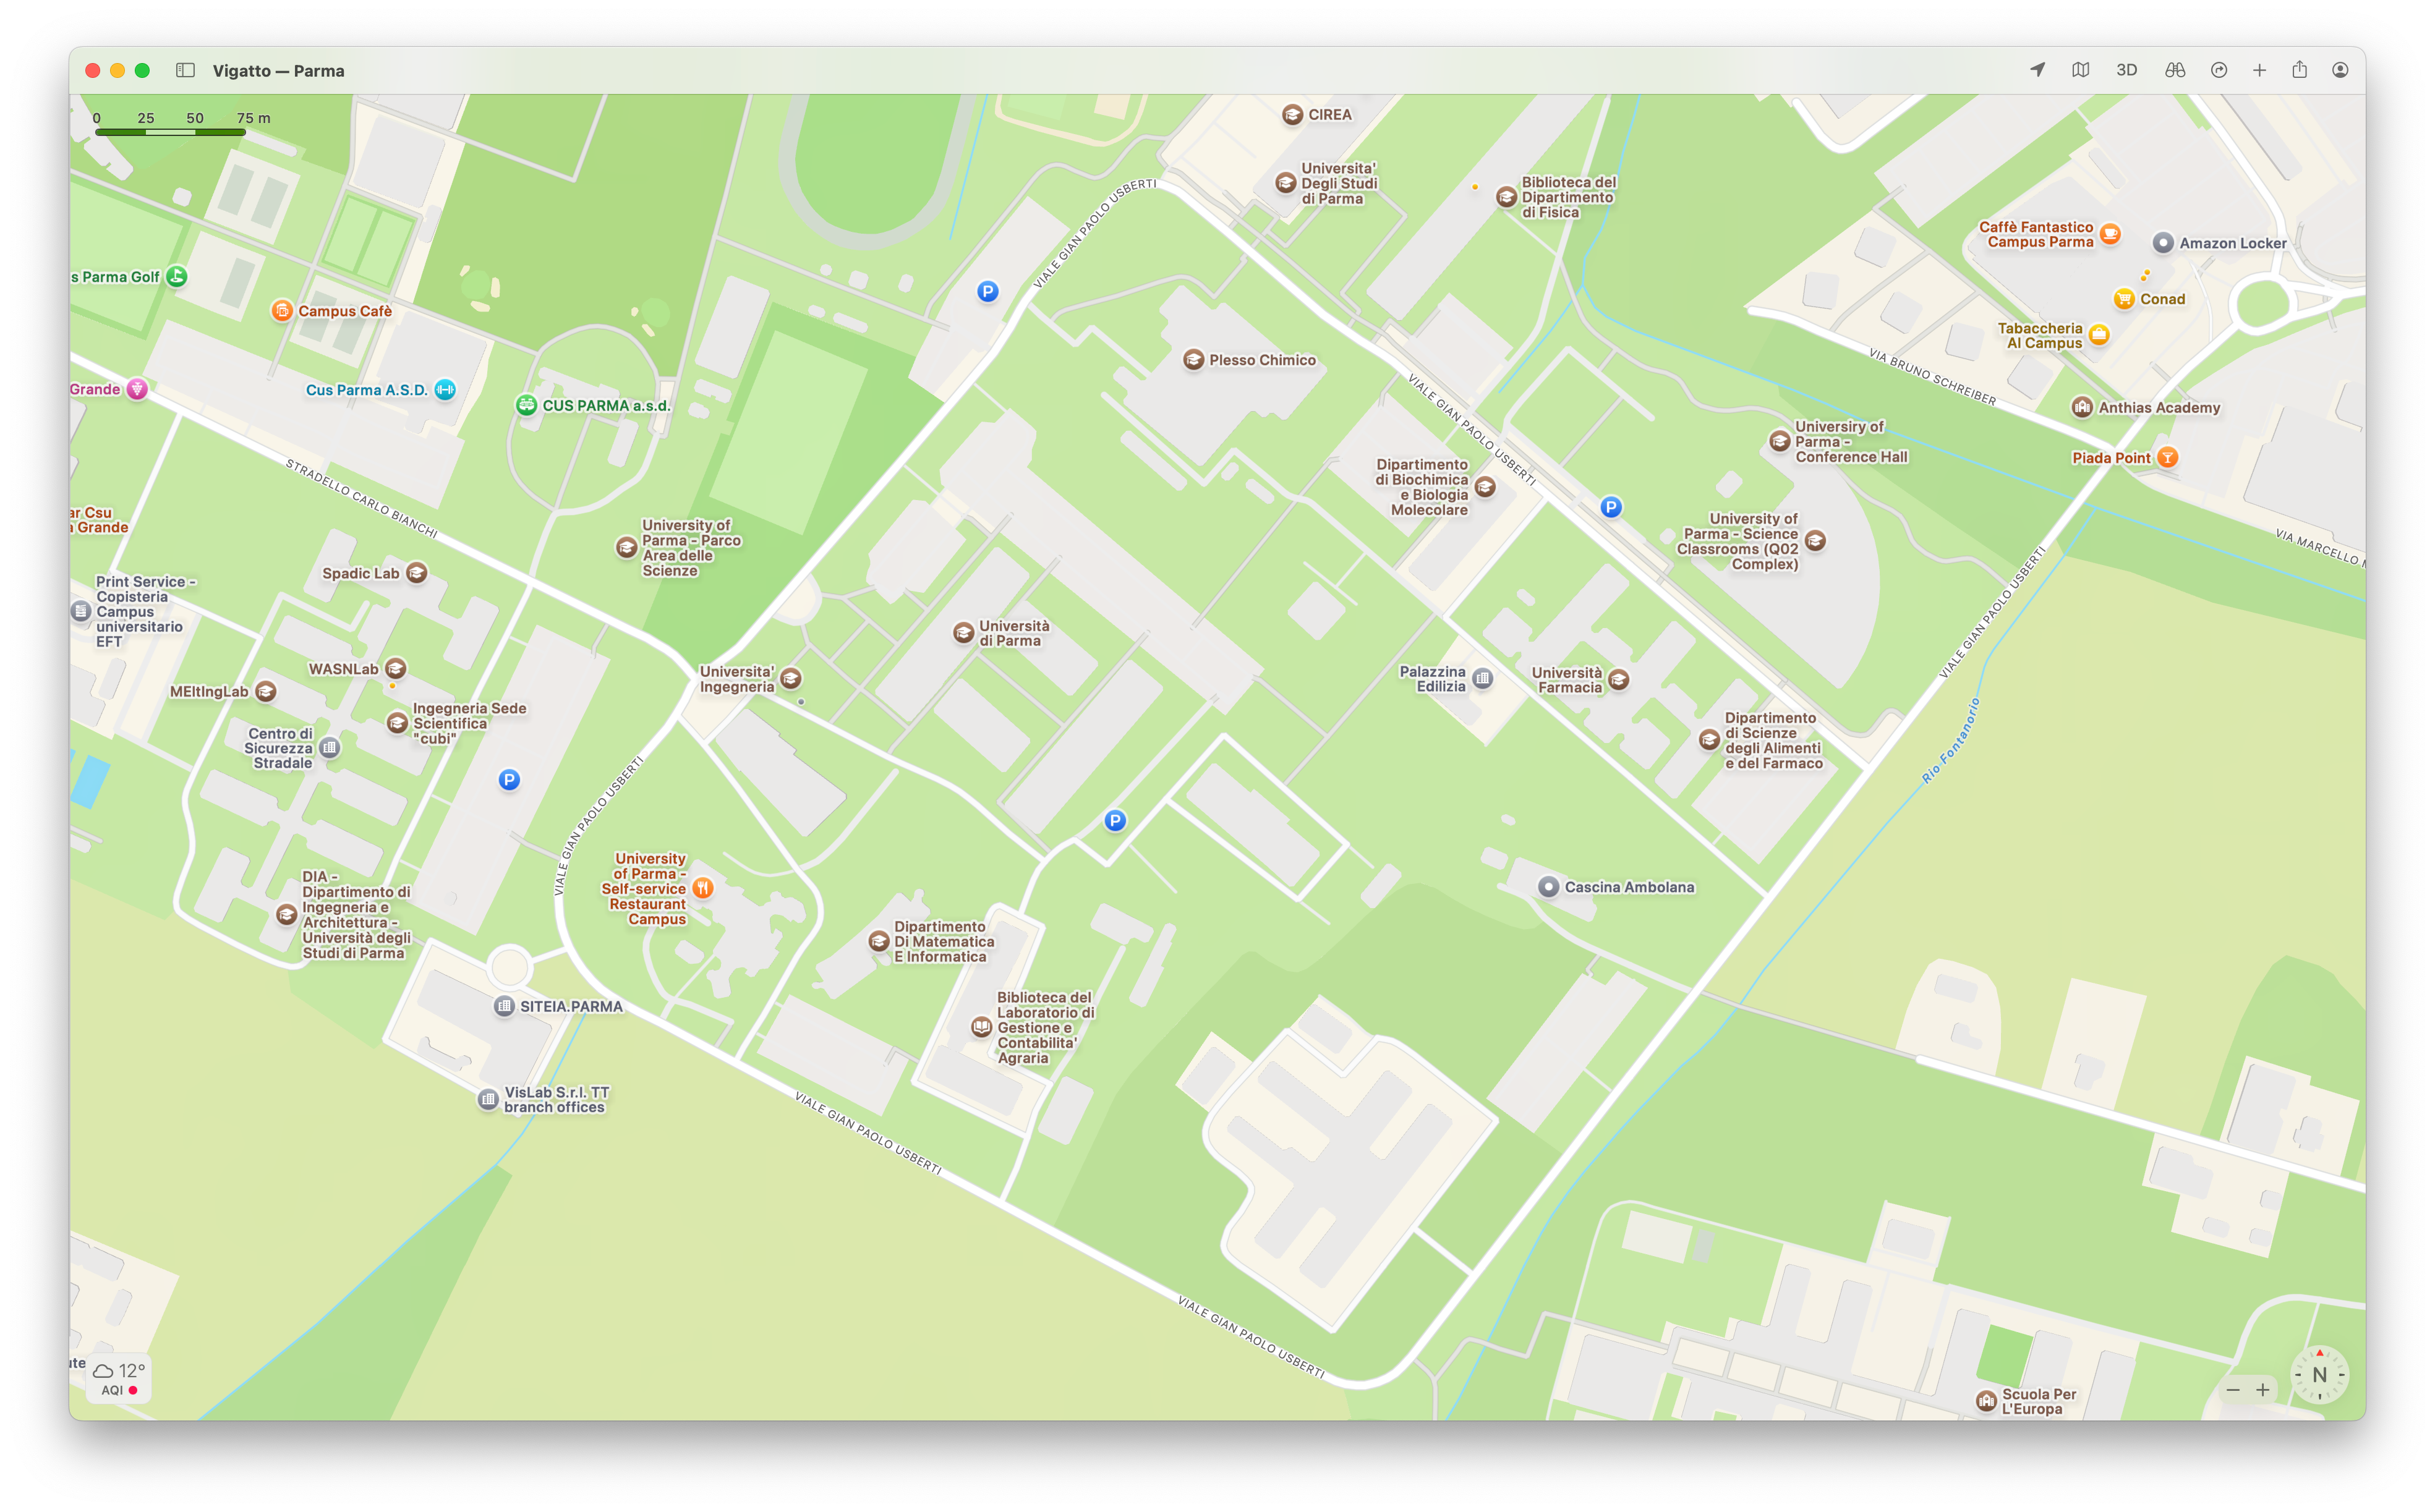
\includegraphics[width=0.65\linewidth]{LateX//figs/SD_MAP.pdf}
    \caption{Illustration of an SD map showcasing its limitations in providing the fine-grained details.}
    \label{fig:sd_map}
\end{figure}
However, SD maps alone are not enough for autonomous driving, where a vehicle must take decisions independently and requires a clear sense of its environment, they lack the fine-grained detail and real-time data necessary for the complex decision-making required in this field.

\subsection{Topological Maps}
Topological maps, which are representations of a space that emphasizes the connectivity and relationships between different locations rather than their exact distances or physical layout, began to be explored around the 2000s. They introduce a layer of connectivity that can be helpful in robot navigation. These maps represent environments through a graph structure, where intersections, pathways, and connections between road segments are shown without needing precise geometric data \cite{li2020survey}. For example, a topological map of a subway system uses nodes to represent stations, with edges representing navigable paths between them \cite{8105770}.
Topological maps provide advantages by saving only relevant information at points called nodes, which represent specific situations, places, or landmarks. They require less memory than metric maps, which memorizes every pixel in the environment. These nodes are connected by edges, defining navigable paths between locations, and can store useful data, such as poses and scans, to aid in localization \cite{murciego2021topological}.

\subsection{HD Maps}
High-Definition (HD) Maps play a crucial role in autonomous driving by providing highly accurate and detailed information about the road and its surroundings. These maps are specifically designed to support navigation and decision-making for self-driving vehicles.

Unlike traditional maps, HD Maps include semantic information, such as labeled features for lanes, traffic signals, pedestrian zones, and other road elements. This functional context can help understand road rules and identify specific areas with precision. With centimeter-level accuracy \cite{geospatialworld_hd_maps}, combining data from both topological and semantic maps, HD Maps can guarantee precise localization and path planning, as illustrated in Figure~\ref{fig:hd_map}.
\begin{figure}[H]
    \centering
    \includegraphics[width=1\linewidth]{LateX//figs/CAP1_MERGE_HD_MAP.pdf}
    \caption{An example of an HD Map that combines topological and semantic information.}
    \label{fig:hd_map}
\end{figure}

The idea of HD Maps began with Mercedes-Benz in 2010 and gained attention in 2013 with the Bertha Drive Project. In this project, a fully autonomous Mercedes-Benz S500 successfully traveled the historic Bertha Benz Memorial Route using a highly accurate 3D map. This project, in partnership with the mapping company HERE, led to the development of the HD Live Map \cite{8105770}.
HD Maps are crucial for autonomous driving because they allow vehicles to pinpoint their position on the road, even in busy urban areas where satellite signals might be weak, due to multi-path fading issues, or inaccurate.

With recent improvements in computing and sensor technology, onboard systems, using cameras, LiDAR, GNSS-IMU (INS), and other sensors, can now process large amounts of data in real-time. These sensors allow the vehicle to handle key tasks such as positioning, mapping, perception, planning movements, and control. When paired with HD maps, these provide autonomous vehicles with crucial information to improve awareness of the surroundings and ensure safety.
HD maps go beyond basic navigation; they function as an additional \textit{sensor} for the vehicle, providing crucial support when other sensors may be less reliable due to certain weather conditions, like sunlight affecting cameras or light rain impacting radar\cite{edmap_2004}.

For HD maps, to be effective in autonomous driving, they must meet certain standards:
\begin{enumerate}
    \item High accuracy: HD maps need sub-meter precision to ensure exact positioning.
    \item 3D representation: All map features should be accurately mapped in all three dimensions;
    \item Detailed attributes: Road elements such as lanes, boundaries, and signs must be clearly defined with attribute data;
    \item Real-world scale consistency: HD maps must precisely match real-world measurements, with no tolerance for scale errors;
    \item Dynamic data: HD maps should include dynamic information to support the vehicle’s decisions during driving.
\end{enumerate}

Today, several companies provide HD mapping services for autonomous driving systems. For instance, the TomTom HD Map \cite{TomTomHDMaps} allows vehicles to locate their position on the road with centimeter-level accuracy. TomTom’s RoadDNA, as shown in Figure~\ref{fig:road_dna}, improves this accuracy further by offering localization layers that work well with various sensor setups, providing data in formats that enhance a vehicle’s understanding of its environment.
\begin{figure}
    \centering
    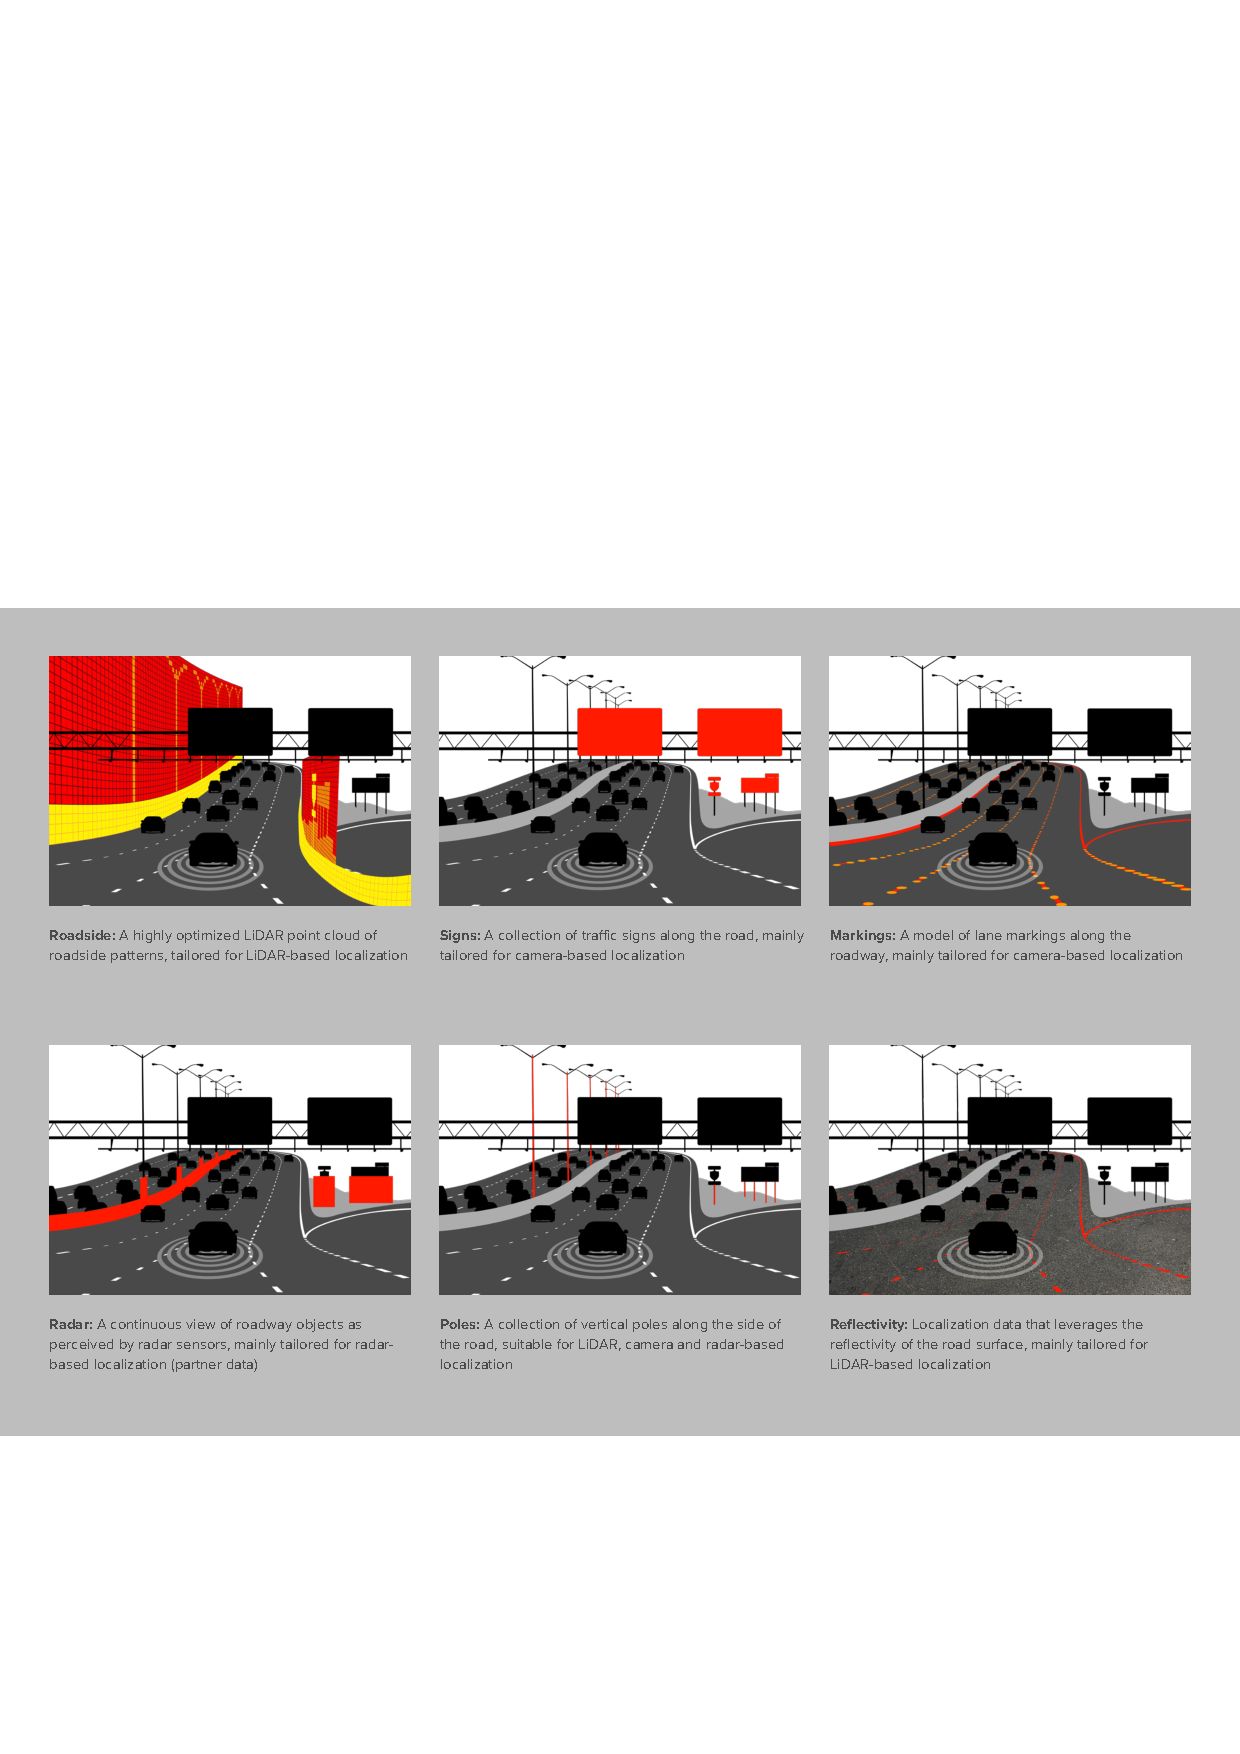
\includegraphics[width=0.9\linewidth]{LateX//figs/HD-Map-with-RoadDNA-Product-Sheet.pdf}
    \caption{Illustration of TomTom’s HD Map and RoadDNA, showcasing its localization layers and data formats that enhance autonomous vehicle positioning and environment understanding \cite{TomTomHDMaps}.}
    \label{fig:road_dna}
\end{figure}

Similarly, HERE and others maps companies, offers an HD Live Map service, which includes detailed, real-time data layers, allowing autonomous vehicles to safely navigate complex routes.

In simple terms, HD maps are highly detailed 3D reconstructions of the road environment, encompassing features such as connections between lanes (including implied ones), lane markings, curbs, traffic signs, pedestrian crossings, traffic lights linked to lanes, and altitude information. 

Their primary advantages include their exceptional level of detail, their ability to function as an additional sensor when onboard sensors are insufficient (e.g., during severe weather conditions), and their provision of all the semantic information required by an autonomous vehicle.

The main challenge of high-definition (HD) maps is their complexity and the high cost of maintenance and updates. Mapping large areas, such as entire highway networks needed for widespread vehicle deployment, requires significant resources. For auto-makers, keeping maps up-to-date can become a major expense, as accurate maps are essential for effective operation \cite{gitlin2017detailedmaps}. Highway networks in regions like Central and Western Europe cover hundreds of thousands of kilometers. Even after the initial mapping is complete, these maps quickly become outdated due to road changes and construction. Autonomous systems depending on HD maps need frequent updates, ideally every few weeks, compared to standard maps for human drivers, which may take months to refresh. This creates a significant challenge for HD map providers to maintain quality while ensuring frequent updates.

Currently, most HD mapping companies use specialized survey vehicles equipped with advanced sensors to collect data. However, deploying enough vehicles to keep maps current over large regions, such as the U.S. or Europe, remains a logistical and financial challenge \cite{dahlstrom2021hdmaps}.

Combining real-time data from vehicle sensors with cloud-based HD map data creates a virtual representation of the environment, including landmarks. However, this process faces several technical bottlenecks:
\begin{itemize}
    \item \textit{Data collection:} Driving for just one hour generates massive amounts of data, requiring significant storage and processing capacity;
    \item \textit{Data processing:} Turning raw data into usable navigation information is computationally intensive and can take days;
    \item \textit{Data transmission:} Current network speeds are insufficient to handle the large data volumes efficiently, even with emerging technologies like 5G;
    \item \textit{Latency:} Real-time operation demands extremely low latency, requiring high-performance onboard computing.
\end{itemize}

These challenges emphasize the need for a balanced approach, integrating external HD map data with the autonomous vehicle's onboard capabilities \cite{SEIF2016159, bao2022highdefinitionmapgenerationtechnologies}.

Autonomous vehicles are equipped with advanced sensors that can reconstruct their surroundings in real time. This capability introduces a promising idea: creating HD maps directly onboard the vehicle without depending on external map providers. This approach offers several benefits:
\begin{itemize}
    \item Removes the cost of purchasing and maintaining external HD maps;
    \item Avoids reliance on frequent external updates;
    \item Reduces dependency on third-party providers, lowering risks of data corruption or security issues.
\end{itemize}

A neural network architecture can be developed to enable real-time HD map reconstruction. Recent approaches, such as \textit{HDMapNet} \cite{li2022hdmapnetonlinehdmap}, use neural networks to reconstruct HD maps from sensor data captured by the vehicle. These systems focus on dynamically building semantic maps based on observations from onboard sensors. HDMapNet, for instance, combines image features from vehicle cameras and point clouds from LiDAR to predict map elements in bird's-eye view, like it can be seen in Figure ~\ref{fig:hd_map_net}.
\begin{figure}[H]
    \centering
    \includegraphics[width=1\linewidth]{LateX//figs/HDmapNET.pdf}
    \caption{In contrast to pre-annotating global semantic maps, a local map learning framework is presented that makes use of on-board sensors to estimate local semantic maps \cite{li2022hdmapnetonlinehdmap}.}
    \label{fig:hd_map_net}
\end{figure}

To train such neural networks effectively, accurate ground truth data is indispensable. In this context, ground truth refers to the precise segment of the HD map that must be reconstructed from the raw data collected by the vehicle's sensors. Achieving this requires exact localization to align the sensor data with the corresponding HD map. This thesis contributes to this process by automating the creation of training datasets. The proposed method selects ground truth data for the network's target predictions using an offline localization method with high accuracy. By automating this step, the dataset creation pipeline becomes more efficient, enabling faster data processing and analysis. This, in turn, allows the model to train with larger datasets, improving its robustness and scalability over time.

\section{Localization on HD Maps: A State-of-the-Art Review}

Localization is a fundamental subsystem in autonomous vehicles, directly impacting the accuracy and reliability of high-definition (HD) maps. The most common techniques for localization integrate data from multiple sensors, including GNSS, IMU, cameras, LiDAR, and radar, in conjunction with HD maps. These techniques can broadly be classified into odometry-based methods, map matching algorithms, and fusion-based approaches.

Odometry-based methods, such as visual odometry and LiDAR odometry, estimate a vehicle's motion by comparing consecutive sensor readings. Techniques like Visual SLAM \cite{10353965} and LiDAR SLAM \cite{9707054} build on these methods by adding features like loop closure and optimization, which help improve accuracy over time. However, these methods often require significant computational power, especially in environments with many features or dense structures. One limitation of these methods is that they do not use a pre-existing map. This means the vehicle cannot anticipate road details, which can be a problem in challenging conditions such as bad weather or when parts of the road are blocked or obscured.

Map matching algorithms align a vehicle's estimated path with features in an HD map. These algorithms can work in two modes: online, for real-time localization, and offline, for high-accuracy tasks such as creating or updating HD maps. 
Geometric techniques, such as point-to-curve and curve-to-curve matching, are the basic methods used in map matching. Modern approaches improve these techniques by using \textit{Lanelet maps} \cite{6856487}, which represent the drivable environment with both geometric and topological details like in Figure~\ref{fig:lanelet-map}. Lanelets are small, connected road segments that can include additional information about the static environment. Vectorized HD maps are also used to improve accuracy in map matching by representing data, not as a grid of pixels (raster), rather as geometric primitives such as points, lines, curves, and polygons.
\begin{figure}[H]
    \centering
    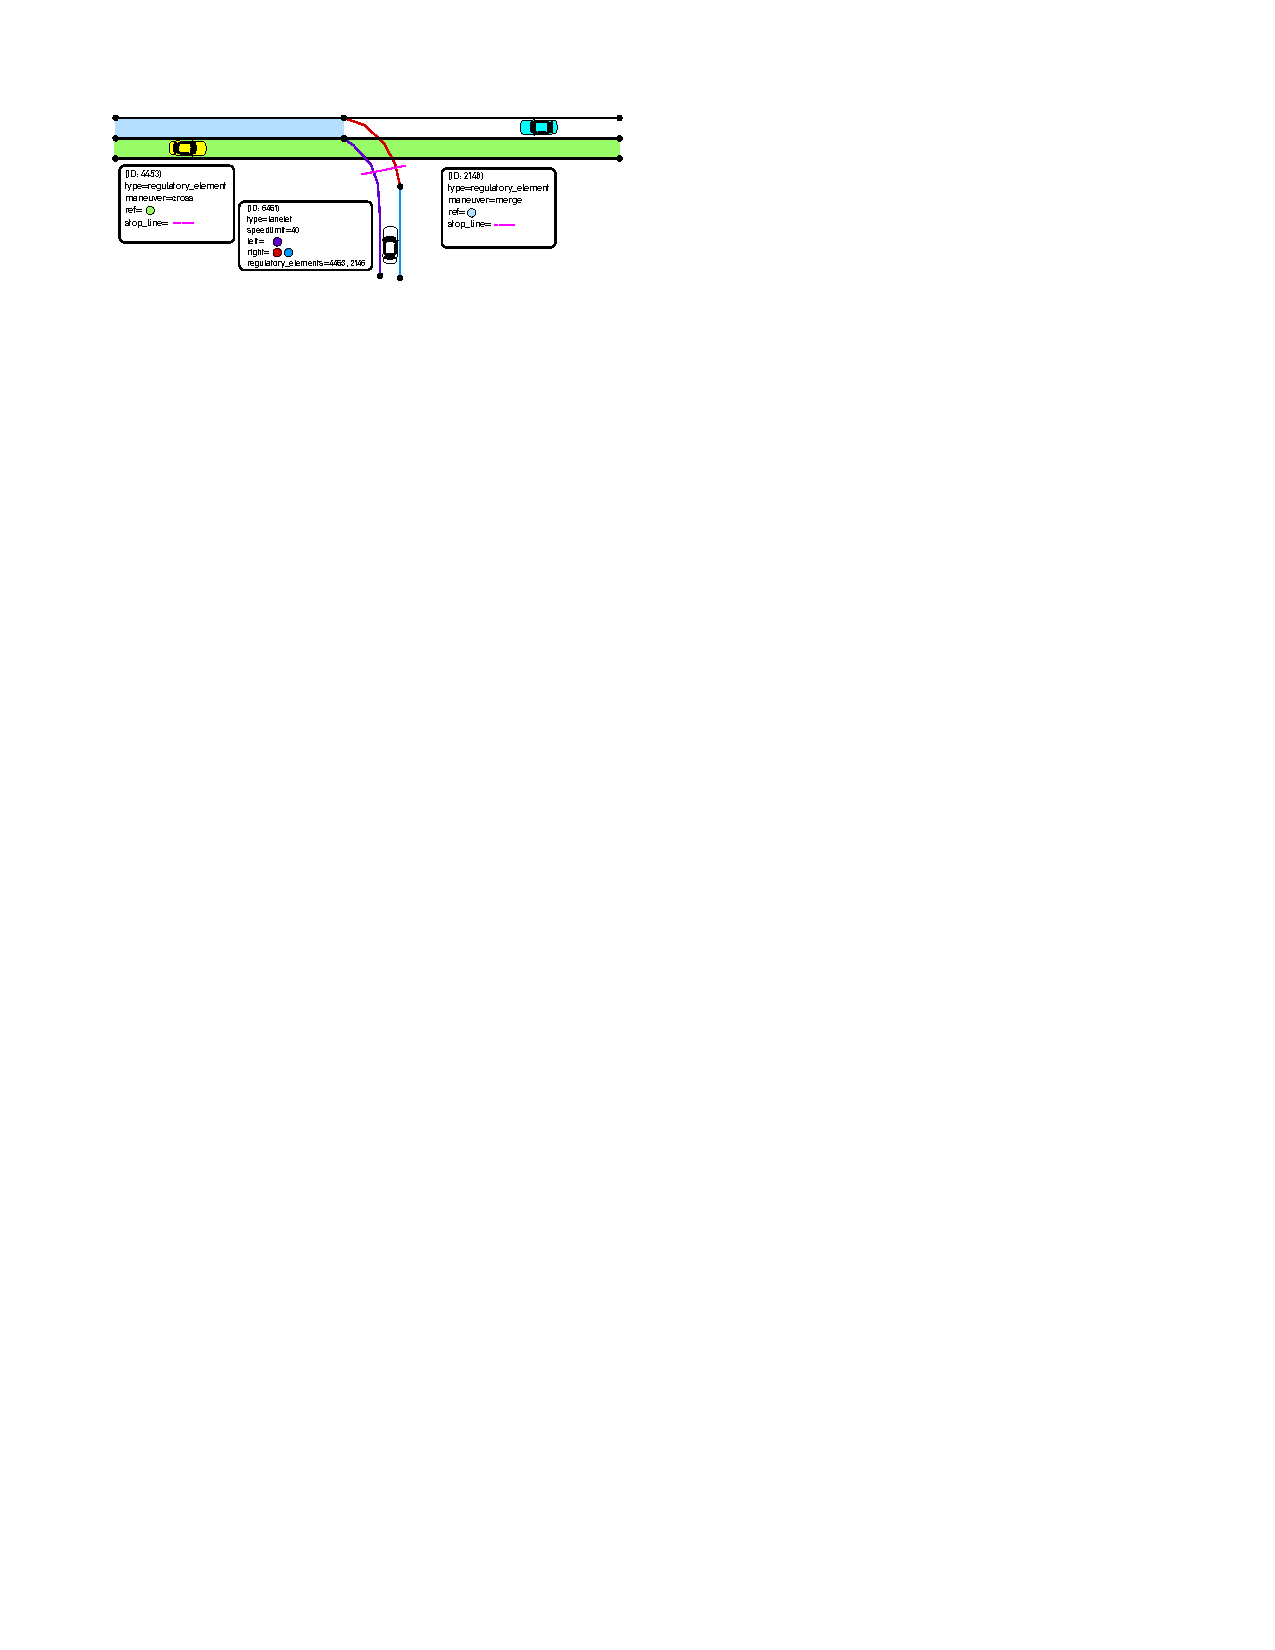
\includegraphics[width=0.75\linewidth]{LateX//figs/Lanelets_Efficient_map_representation_for_autonomous_driving.pdf}
    \caption{Lanelet maps: an efficient representation of the drivable environment for autonomous driving \cite{6856487}.}
    \label{fig:lanelet-map}
\end{figure}

Fusion-based approaches combine data from multiple sensors, such as GNSS, IMU, LiDAR, and cameras, with HD map features. These methods use filtering techniques (e.g., Kalman Filters) and optimization frameworks to improve localization robustness and accuracy, even in challenging environments with occlusions or poor GNSS signals. 

This section explores the state of the art in localization methods, with a focus on offline approaches that are crucial for this thesis \cite{Liu_Wang_Zhang_2020, wijaya2024highdefinitionmapmapping}. Localization in autonomous driving often involves recording data from the ego vehicle's sensors and compare them to ones from an HD map in order to estimate its pose. One common data format used in such tasks is the point cloud\footnote{A point cloud is a collection of 3D data points obtained from sensors like LiDAR or stereo cameras, representing locations in space and possibly additional attributes such as intensity or color.}. 

Point cloud registration is the process of aligning an input scan \( S \) (source) with a map \( M \) (target). Common algorithms for this task include the Iterative Closest Point (ICP) and Normal Distributions Transform (NDT). 

Although this work focuses on offline methods, other types of data and techniques will be discussed in the following sections.

\subsection*{Iterative Closest Point (ICP)}
The first point cloud matching algorithm presented is the Iterative Closest Point (ICP) \cite{s20082166, Liu_Wang_Zhang_2020}. ICP treats the registration problem as an iterative optimization process It establishes correspondences between the nearest points in \( S \) and \( M \) and minimizes the sum of squared distances between these correspondences as shown in Figure~\ref{fig:icp_matching}. 
\begin{figure}[H]
    \centering
    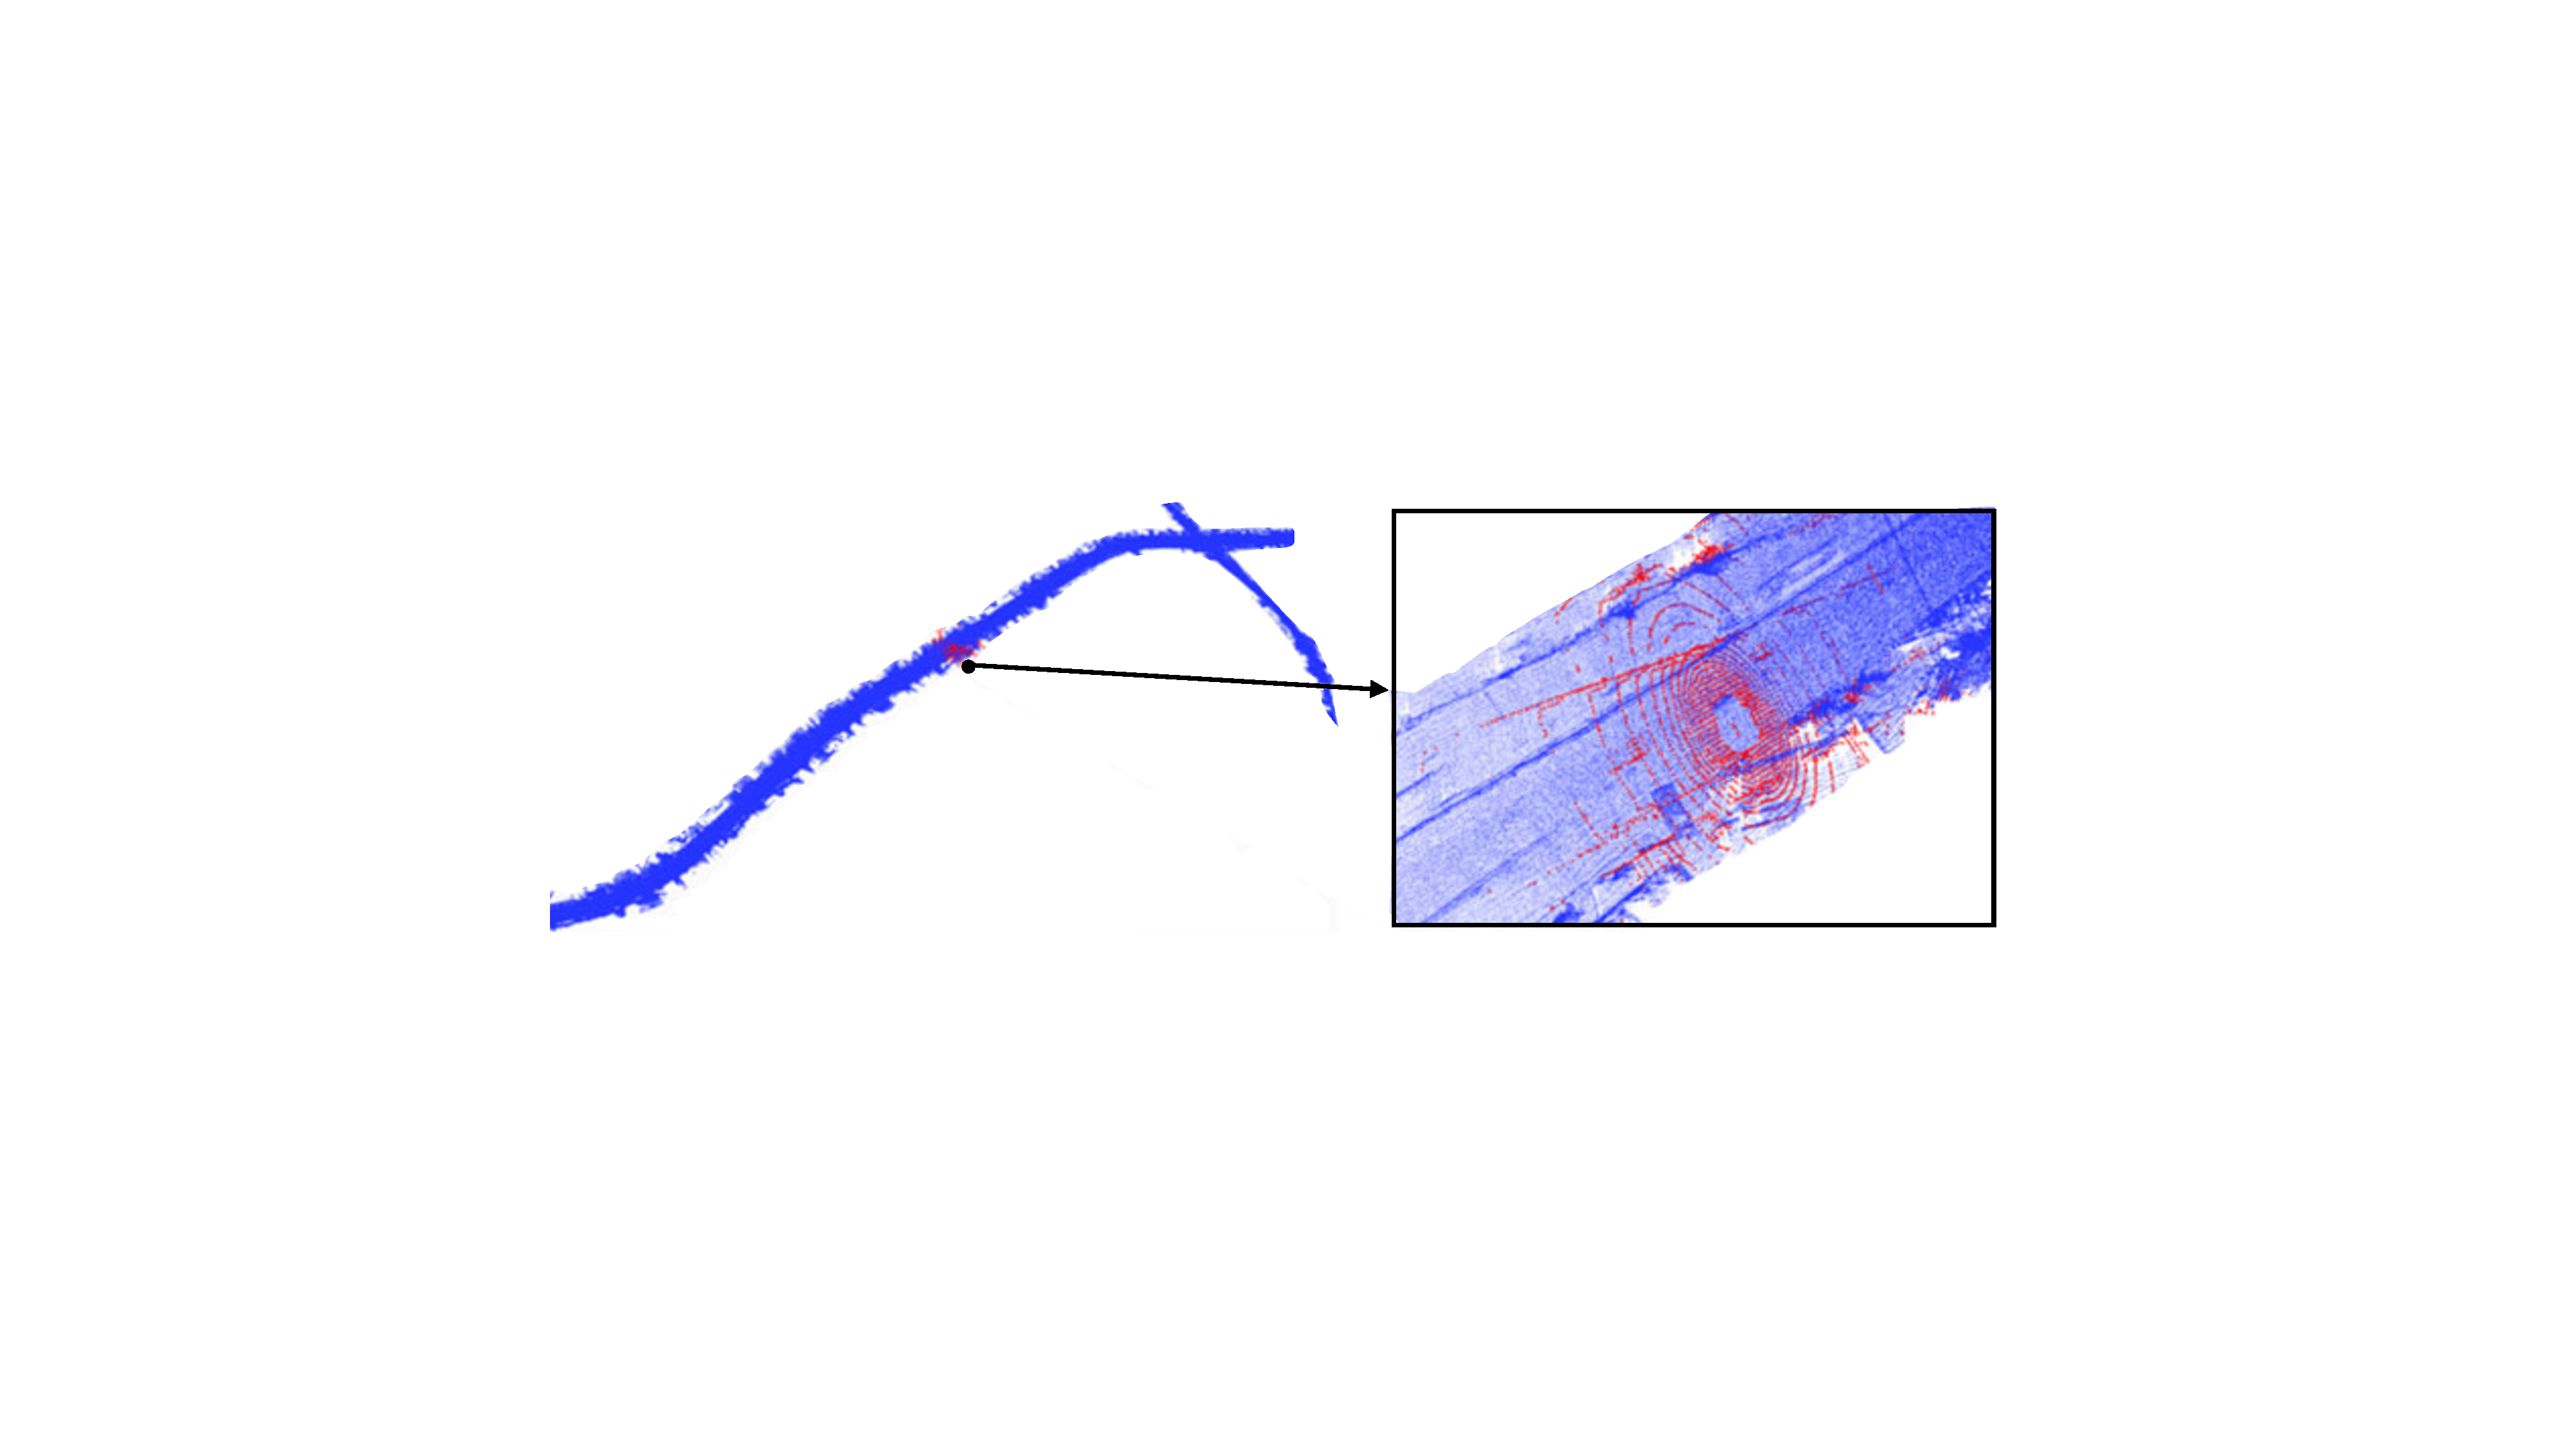
\includegraphics[width=1\linewidth]{LateX//figs/icp.pdf}
    \caption{The 3D point-cloud based HD map and a section with matched scan reported in red.}
    \label{fig:icp_matching}
\end{figure}

The optimization problem can be expressed as:
\begin{equation}
    \min_{\mathbf{T}} \sum_{i=1}^{N_s} \| \mathbf{T} \mathbf{x}_i - \mathbf{y}_{\text{nearest}}(\mathbf{x}_i) \|^2,
\end{equation}

where \( \mathbf{T} \in SE(3) \) is the rigid-body transformation matrix, \( \mathbf{x}_i \) are the points in the source scan \( S \), and \( \mathbf{y}_{\text{nearest}}(\mathbf{x}_i) \) represents the nearest point in \( M \) corresponding to \( \mathbf{x}_i \). 
The ICP algorithm alternates between two steps:
\begin{enumerate}
    \item \textit{Correspondence assignment:} Find the nearest neighbors between \( S \) and \( M \);
    \item \textit{Pose update:} Solve for the transformation \( \mathbf{T} \) that minimizes the alignment error.
\end{enumerate} 
The main drawbacks of this approach are:
\begin{itemize}
    \item \textit{Sensitive to Initial Guess}: ICP needs a good starting alignment of the two shapes. If the initial positions are far apart, the algorithm might not work well and could get stuck in a wrong solution;
    \item \textit{Slow for Large Data}: When dealing with very large point clouds, ICP can take a lot of time because it has to match every point in one set to the closest point in the other set repetitively;
    \item \textit{Prone to Local Minima}: ICP might not find the best alignment if there are multiple possible alignments. Instead, it may stop at a sub-optimal solution (a \textit{local minimum});
    \item \textit{Assumes Similarity}: ICP works best when the two shapes being aligned are already similar. If there are large differences (like missing parts due to obstruction or noise), the algorithm might fail;
    \item \textit{Sensitive to Noise and Outliers}: Points that don’t belong to the object (outliers) or errors in the data (noise) can cause the alignment to be inaccurate.
\end{itemize}

\subsection*{Normal Distributions Transform (NDT)}
The second matching algorithm presented is NDT \cite{5353908, Liu_Wang_Zhang_2020} which takes a probabilistic approach by discretizing the map \( M \) into a grid of cells \( \ \beta_i \ \) and modeling the points within each cell as a Gaussian distribution. For each cell \( \beta_i \), the mean vector \( \boldsymbol{\mu}_i \) and covariance matrix \( \Sigma_i \) are computed as:
\begin{equation}
    \boldsymbol{\mu}_i = \frac{1}{n_i} \sum_{k=1}^{n_i} \mathbf{z}_k, \quad
    \Sigma_i = \frac{1}{n_i - 1} \sum_{k=1}^{n_i} (\mathbf{z}_k - \boldsymbol{\mu}_i)(\mathbf{z}_k - \boldsymbol{\mu}_i)^\top,
\end{equation}
where \( \mathbf{z}_k \) are the points in cell \( \beta_i \), and \( n_i \) is the number of points in the cell.
The likelihood of a point \( \mathbf{x}_i \) from \( S \) belonging to a cell \( \beta_i \) in \( M \) is evaluated using the multivariate Gaussian probability density function:
\begin{equation}
    p(\mathbf{x}_i | \beta_i) = \frac{1}{(2\pi)^{d/2} |\Sigma_i|^{1/2}} \exp\left(-\frac{1}{2} (\mathbf{x}_i - \boldsymbol{\mu}_i)^\top \Sigma_i^{-1} (\mathbf{x}_i - \boldsymbol{\mu}_i)\right)
\end{equation}
The transformation \( \mathbf{T} \) is then optimized to maximize the overall likelihood:
\begin{equation}
    \max_{\mathbf{T}} \sum_{i=1}^{N_s} p(\mathbf{T} \mathbf{x}_i | \beta_{\text{nearest}}(\mathbf{T} \mathbf{x}_i))
\end{equation} 

The whole process can be seen in Figure~\ref{fig:ndt-figure} and in the algorithm shown below:
\begin{figure}[H]
    \centering
    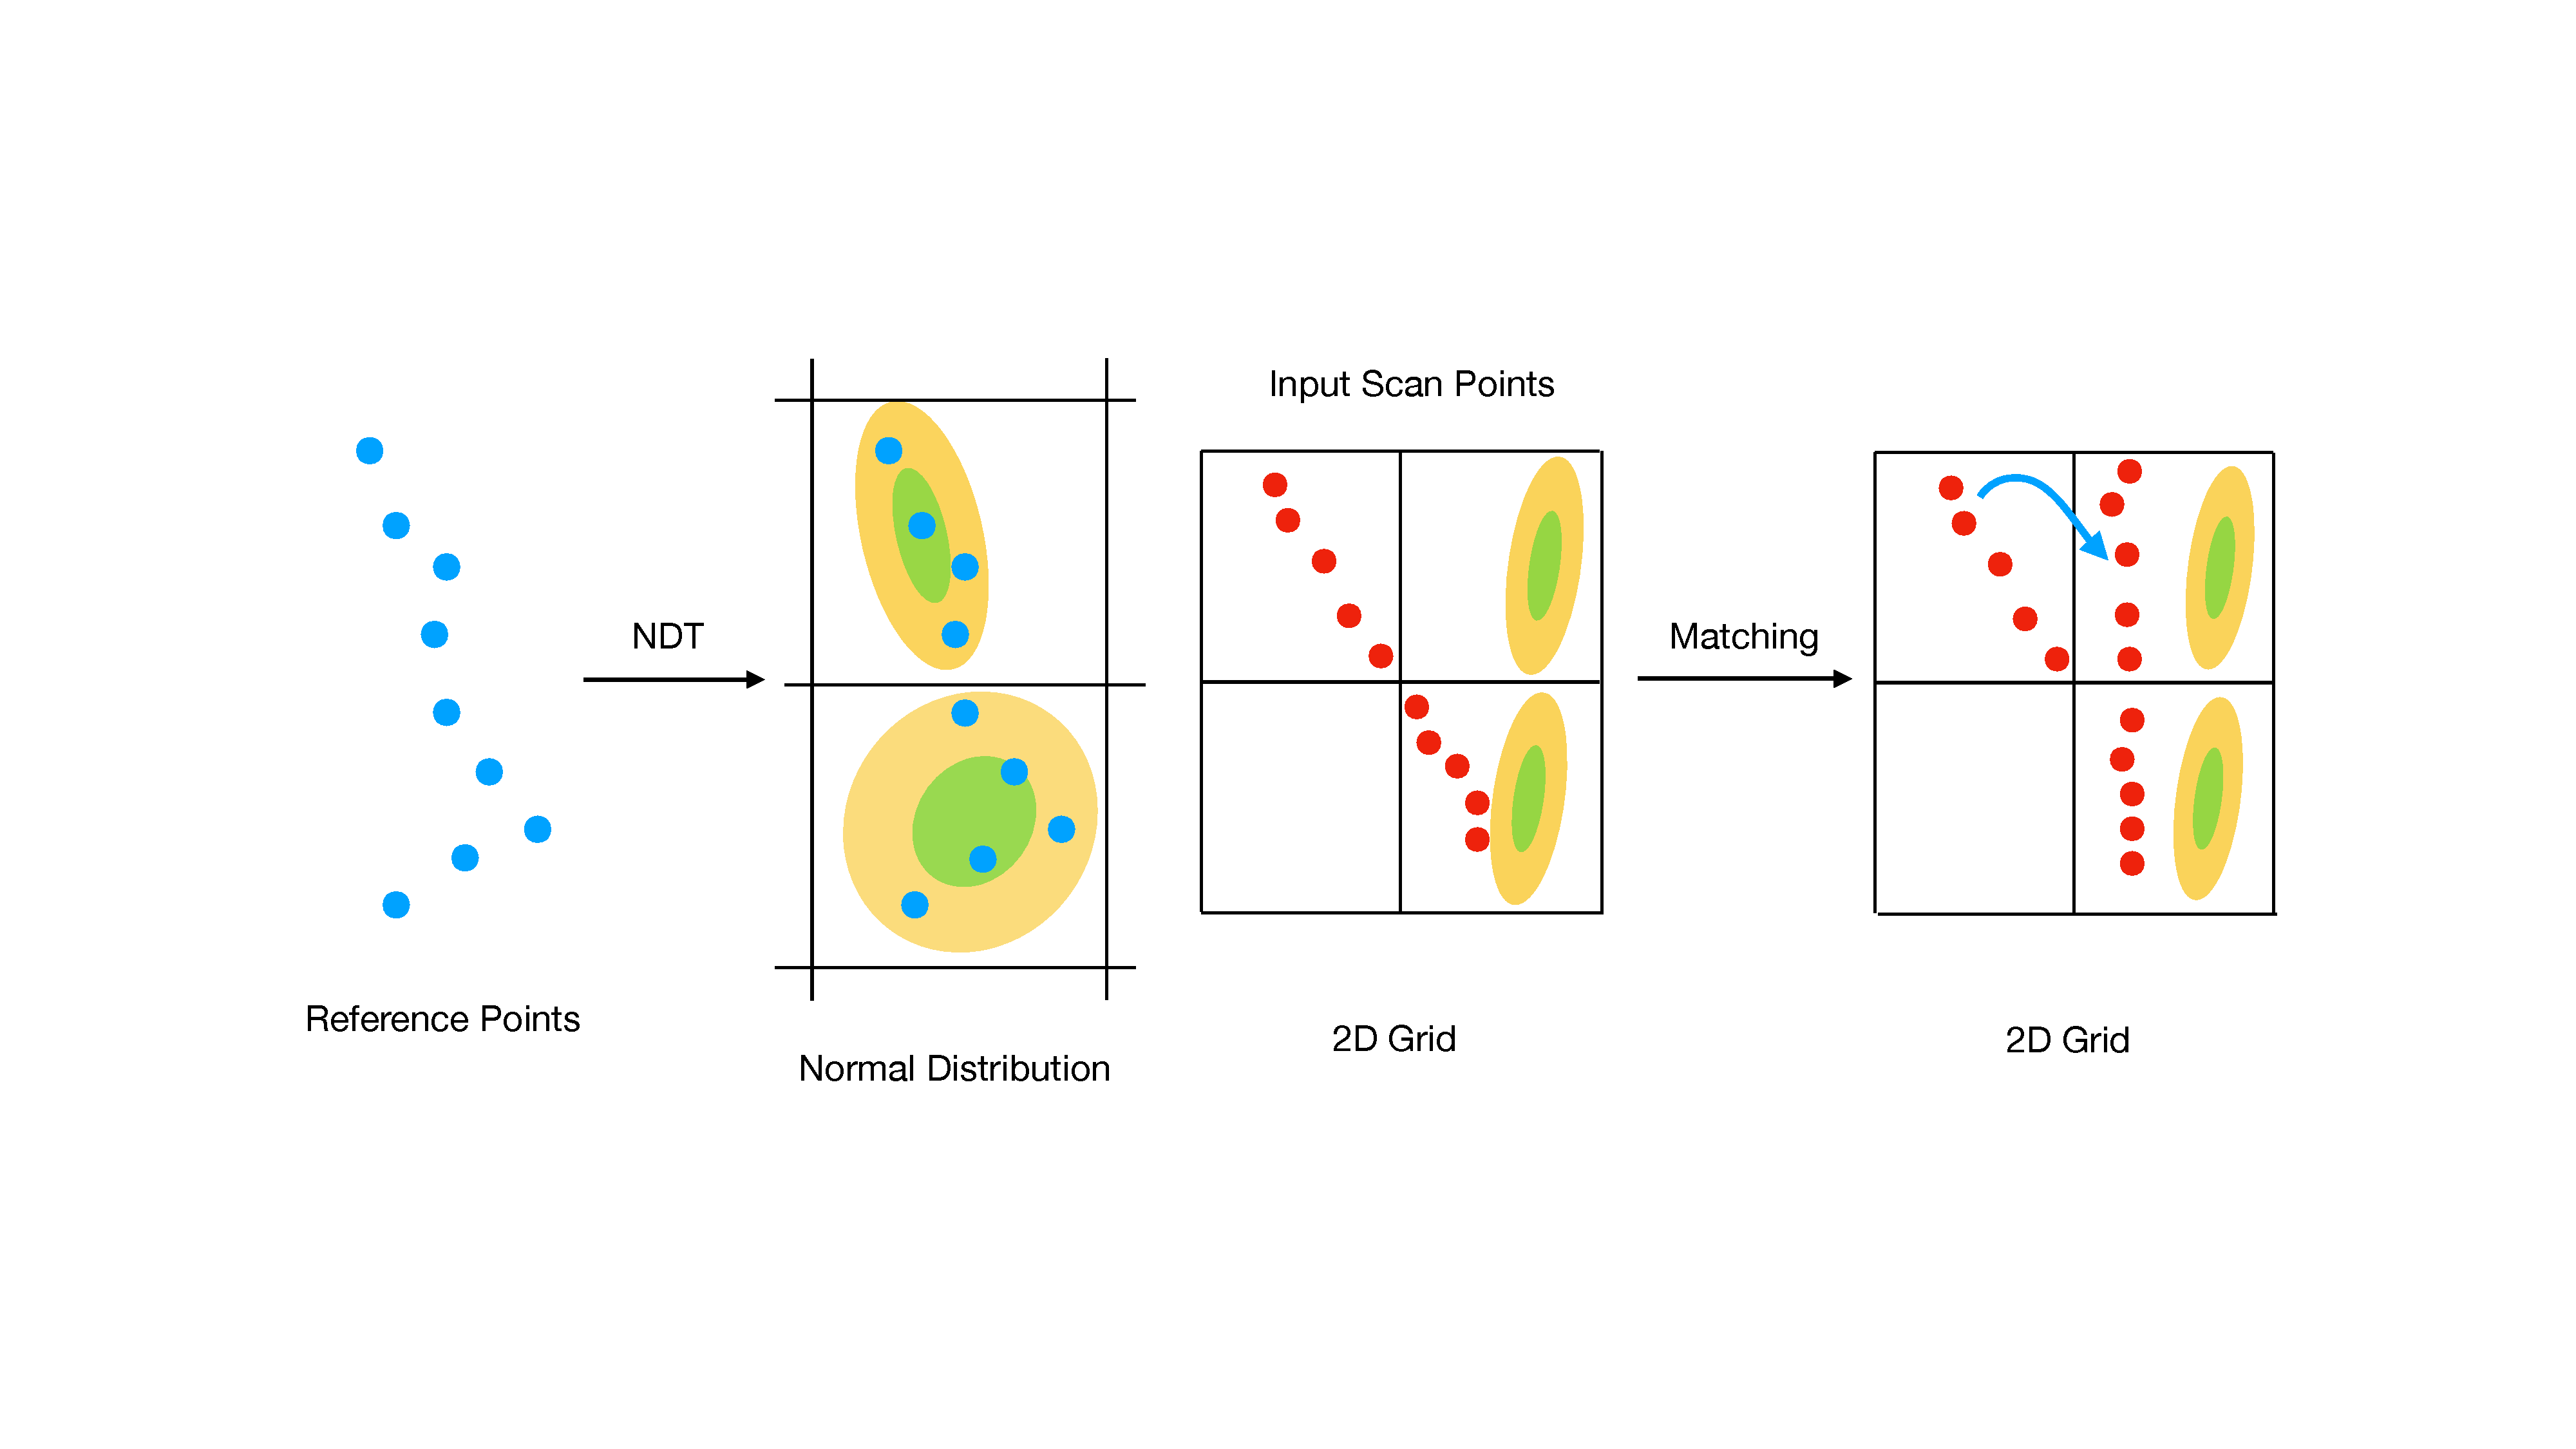
\includegraphics[width=1\linewidth]{LateX//figs/ndt.pdf}
    \caption{Normal Distributions Transform (NDT) \cite{5353908}. This figure illustrates the steps of the NDT process: alignment of point clouds using probability density functions.}
    \label{fig:ndt-figure}
\end{figure}

\begin{algorithm}[H]
\caption{Normal Distributions Transform (NDT)}
\begin{algorithmic}[1]
\State \textbf{Input:} Source scan \( S \), map \( M \), initial pose \( \mathbf{T}_0 \), cell size \( c \)
\State \textbf{Output:} Optimal transformation \( \mathbf{T} \)
\State Discretize \( M \) into grid cells of size \( c \)
\For{each cell \( \beta_i \) containing points}
    \State Compute \( \boldsymbol{\mu}_i \) and \( \Sigma_i \)
\EndFor
\State Initialize \( \mathbf{T} = \mathbf{T}_0 \)
\Repeat
    \State Transform \( S \) using \( \mathbf{T} \)
    \State Compute likelihood of each point in \( S \) given nearest cell in \( M \)
    \State Update \( \mathbf{T} \) using a gradient-based optimizer
\Until{Convergence criteria are met}
\State \textbf{Return} \( \mathbf{T} \)
\end{algorithmic}
\end{algorithm}

The main drawbacks of this approach are:
\begin{itemize}
    \item \textit{Sensitive to Initial Alignment}: Like ICP, NDT also depends on a good initial alignment. Poor initial guesses can lead to misalignment or failure to converge.
    \item \textit{Computational Cost}: The algorithm can be computationally expensive, especially for large datasets, as it involves dividing space into grids and performing complex calculations;
    \item \textit{Parameter Tuning}: NDT requires careful tuning of parameters, such as grid size. Improper settings can lead to inaccurate results or slow performance.
    \item \textit{Assumes Gaussian Distribution}: NDT assumes that points within each grid cell follow a Gaussian distribution. This assumption may not hold true in some real-world scenarios, leading to errors;
    \item \textit{Not Robust to Noise}: NDT can struggle with noisy or incomplete data, which can disrupt the formation of accurate Gaussian models.
\end{itemize}

Both ICP and NDT are essential tools for scan matching, with ICP being suitable for fine alignment and NDT offering robustness in environments with noise and sparse data.

\subsection*{Path Optimization Without Point Clouds}

While methods like Iterative Closest Point (ICP) and Normal Distributions Transform (NDT) are effective for point cloud-based alignment, there are alternative approaches that do not rely on point clouds. One such technique involves leveraging data from other sources, such as GNSS and Visual Odometry (VO), to reconstruct and optimize the vehicle's path on an HD map. This approach is particularly useful when point cloud data is unavailable or when computational efficiency is a priority.

To achieve this, several steps are undertaken:
\begin{enumerate}
    \item \textit{Data Acquisition}: Data is collected from the Global Navigation Satellite System (GNSS) or through a combination of GNSS and visual odometry. These data sources provide an initial estimate of the vehicle's path.
    \item \textit{Path Reconstruction}: By analyzing the GNSS or odometry data, a preliminary path of the vehicle is reconstructed on the map. However, this path often contains inaccuracies, such as the vehicle being mapped through parking spots or over curbs—areas that were not actually covered. 
    \item \textit{Manual Correction}: To refine the reconstructed path, an operator provides key points through which the vehicle certainly passed. These points are typically centered within the permissible lane boundaries, guiding the optimizer toward a more accurate solution.
    \item \textit{Optimization Process}: A robust optimization algorithm is applied to align the reconstructed path with the HD map. This involves:
    \begin{itemize}
        \item \textit{Minimizing} the distance between observed map boundaries (e.g., lanes, curbs) and their counterparts on the HD map;
        \item \textit{Enforcing} constraints that ensure the vehicle passes close to the manually specified points;
        \item \textit{Maintaining} relative positional consistency between successive frames, ensuring smoothness in the optimized path.
    \end{itemize}
\end{enumerate}

The result is an optimized position that closely matches the true one of the vehicle. This process ensures that the vehicle’s estimated position aligns with the HD map's features, as illustrated in Figure~\ref{fig:optimized-path}.
\begin{figure}[H]
    \centering
    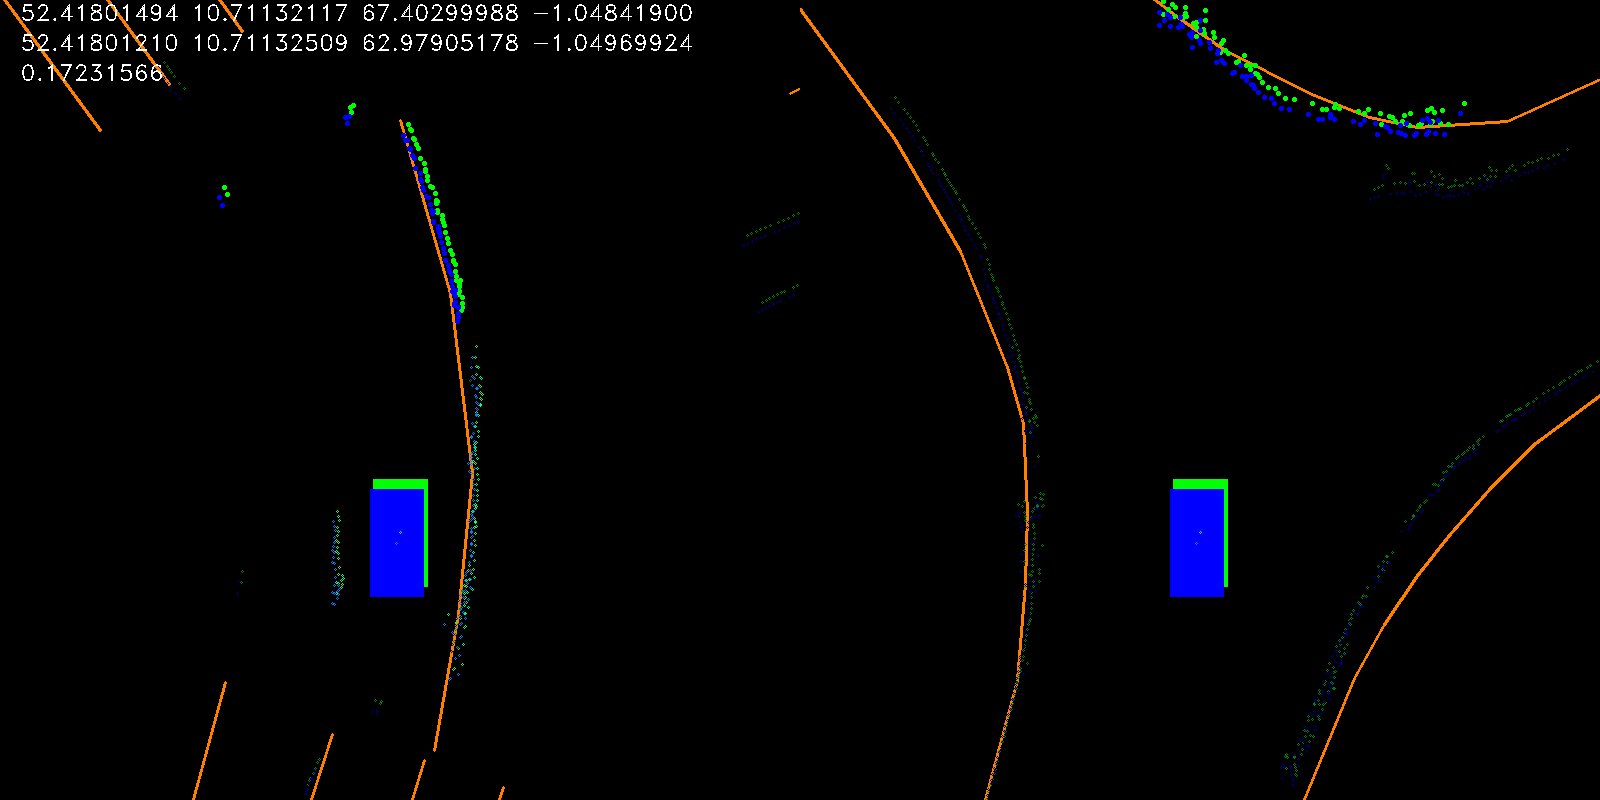
\includegraphics[width=0.75\linewidth]{LateX//figs/opt_pose.png}
    \caption{Optimized vehicle trajectory aligning with HD map features. This figure demonstrates how the estimated position is adjusted to match the ground-truth.}
    \label{fig:optimized-path}
\end{figure}


The operations described can be summarized in the following pseudo-code, and the graphical result can be seen in Figure~\ref{fig:optimizer}:
\begin{algorithm}[H]
\caption{Vehicle Path Optimization on HD Maps}
\begin{algorithmic}[1]
\State \textbf{Input:} GNSS/visual odometry data $\mathcal{D}$, HD map $\mathcal{M}$, manual waypoints $\mathcal{W}$
\State \textbf{Output:} Optimized path $\mathcal{P}_{\text{opt}}$
\State \textbf{Initialize:} Ceres problem $\mathcal{C}$, weights $\lambda$, max iterations $T_{\text{max}}$

\State \textbf{Step 1:} Reconstruct preliminary path $\mathcal{P}_{\text{init}}$ using $\mathcal{D}$.
\State \textbf{Step 2:} Identify keyframes $\mathcal{F}$:
\For {each frame $f_i \in \mathcal{D}$}
    \If {frame is a manual waypoint $w_i \in \mathcal{W}$}
        \State Add $f_i$ to $\mathcal{F}$
    \EndIf
\EndFor

\State \textbf{Step 3:} Add constraints to $\mathcal{C}$:
\For {each frame $f_i \in \mathcal{F}$}
    \If {$f_i$ has manual waypoints $w_i$}
        \State Add manual pose constraint to $\mathcal{C}$
    \EndIf
    \State Add relative pose constraints to $\mathcal{C}$ between $f_i$ and neighbors
    \State Add perception constraints (e.g., lanes, curbs) to $\mathcal{C}$
\EndFor

\State \textbf{Step 4:} Solve optimization problem:
\State Configure Ceres options with $T_{\text{max}}$, threads, and convergence criteria
\State Solve $\mathcal{C}$ using Ceres solver

\State \textbf{Step 5:} Interpolate poses between keyframes:
\For {each consecutive frame pair $(f_i, f_j) \in \mathcal{F}$}
    \For {each intermediate frame $f_k$ between $f_i$ and $f_j$}
        \State Interpolate pose of $f_k$ using weighted average of $f_i$ and $f_j$
    \EndFor
\EndFor

\State \textbf{Return:} $\mathcal{P}_{\text{opt}}$, the optimized path
\end{algorithmic}
\end{algorithm}

\begin{figure}[H]
    \centering
    \includegraphics[width=0.9\linewidth]{drhxfc.pdf}
    \caption{Illustration of the path optimization process. The figure shows the initial path (orange), manually specified points (green), and the final optimized path (red) overlaid on the HD map.}
    \label{fig:optimizer}
\end{figure}

To address the challenge of aligning the vehicle's estimated trajectory with the HD map and correcting inaccuracies in the reconstructed path, the Ceres Solver \cite{Agarwal_Ceres_Solver_2022} can work properly. Ceres is a robust, open-source non-linear least-squares optimizer widely used in robotics and computer vision. It operates by minimizing the sum of squared residuals between the observed and expected values. In this context, the residuals represent discrepancies such as the distance between the vehicle's estimated path and the HD map features (e.g., lanes, curbs), as well as the differences in relative poses between successive frames. By incorporating constraints like manual waypoints and map observations, Ceres ensures that the optimized trajectory is both accurate and smooth, closely matching the vehicle's true path. 

The same pipeline can be used with other optimizers that could solve this problem include \textit{g2o} \cite{Kummerle_g2o_2011}, a graph-based optimization framework widely used in simultaneous localization and mapping (SLAM), and the \textit{Levenberg-Marquardt} algorithm \cite{Levenberg_LMA_1944, Marquardt_LMA_1963}, a hybrid optimization method combining gradient descent and Gauss-Newton techniques for non-linear least squares. 

Bundle adjustment frameworks \cite{Triggs_BA_1999}, which refine poses and 3D points in structure from motion, can also be adapted for trajectory alignment. Additionally, \textit{GTSAM} (Georgia Tech Smoothing and Mapping) \cite{Dellaert_GTSAM_2012}, a library for factor graph-based optimization, is well-suited for problems requiring trajectory smoothing and constraint handling. Non-linear programming solvers such as \textit{IPOPT} \cite{Wachter_IPOPT_2006} are another option, providing robust constraint management for trajectory refinement. 

\subsection*{Neural Networks for Localization}

In addition to traditional optimization methods, recent advancements in neural network-based algorithms offer a promising alternative for solving trajectory alignment and localization problems. For example, \textit{OrienterNet} \cite{sarlin2023orienternetvisuallocalization2d} shows how neural networks can predict precise orientations and locations directly from visual data.

Unlike many visual localization algorithms that depend on complex 3D point clouds, which are expensive to create, store, and maintain, OrienterNet uses simpler 2D semantic maps. 

The goal is to estimate the absolute 6-DoF pose of an image in the world. Under realistic assumptions, this problem can be simplified to estimating a 3-DoF pose \( \boldsymbol{\xi} = (x, y, \theta) \), where \((x, y) \in \mathbb{R}^2\) represent the location and \(\theta \in (-\pi, \pi]\) denotes the heading angle. The analysis assumes a topocentric coordinate system where the \(x\)-\(y\)-\(z\) axes correspond to East-North-vertical directions.

It is reasonable to assume the direction of gravity is known, a capability humans possess through their inner ear, and which can be estimated by the Inertial Measurement Unit (IMU) embedded in many devices. Additionally, the world is largely planar, with most motion in outdoor environments constrained to a 2D surface. The precise height of the camera can be determined as the distance to the ground using a local SLAM reconstruction.

The input consists of an image \( I \) with known pinhole camera calibration. The image is rectified via a homography computed from the known gravity vector, ensuring that roll and pitch angles comes to zero and the principal axis is horizontal. A rough location \( \boldsymbol{\xi}_{\text{prior}} \) is also provided, which could originate from a noisy GPS reading or a previous localization estimate. This measure can have an error of over $20$ meters which is a realistic scenario for consumer-grade sensors in multi-path environments like urban cities.

Map data is queried from OpenStreetMap (OSM) as a square area centered on \( \boldsymbol{\xi}_{\text{prior}} \), with the size of the area depending on the noise level of the prior. The map data consists of polygons, lines, and points, each annotated with a semantic class and provided in a local reference frame.

OrienterNet comprises three main modules, as illustrated in Figure~\ref{fig:orienternet}:
\begin{figure}[H]
    \centering
    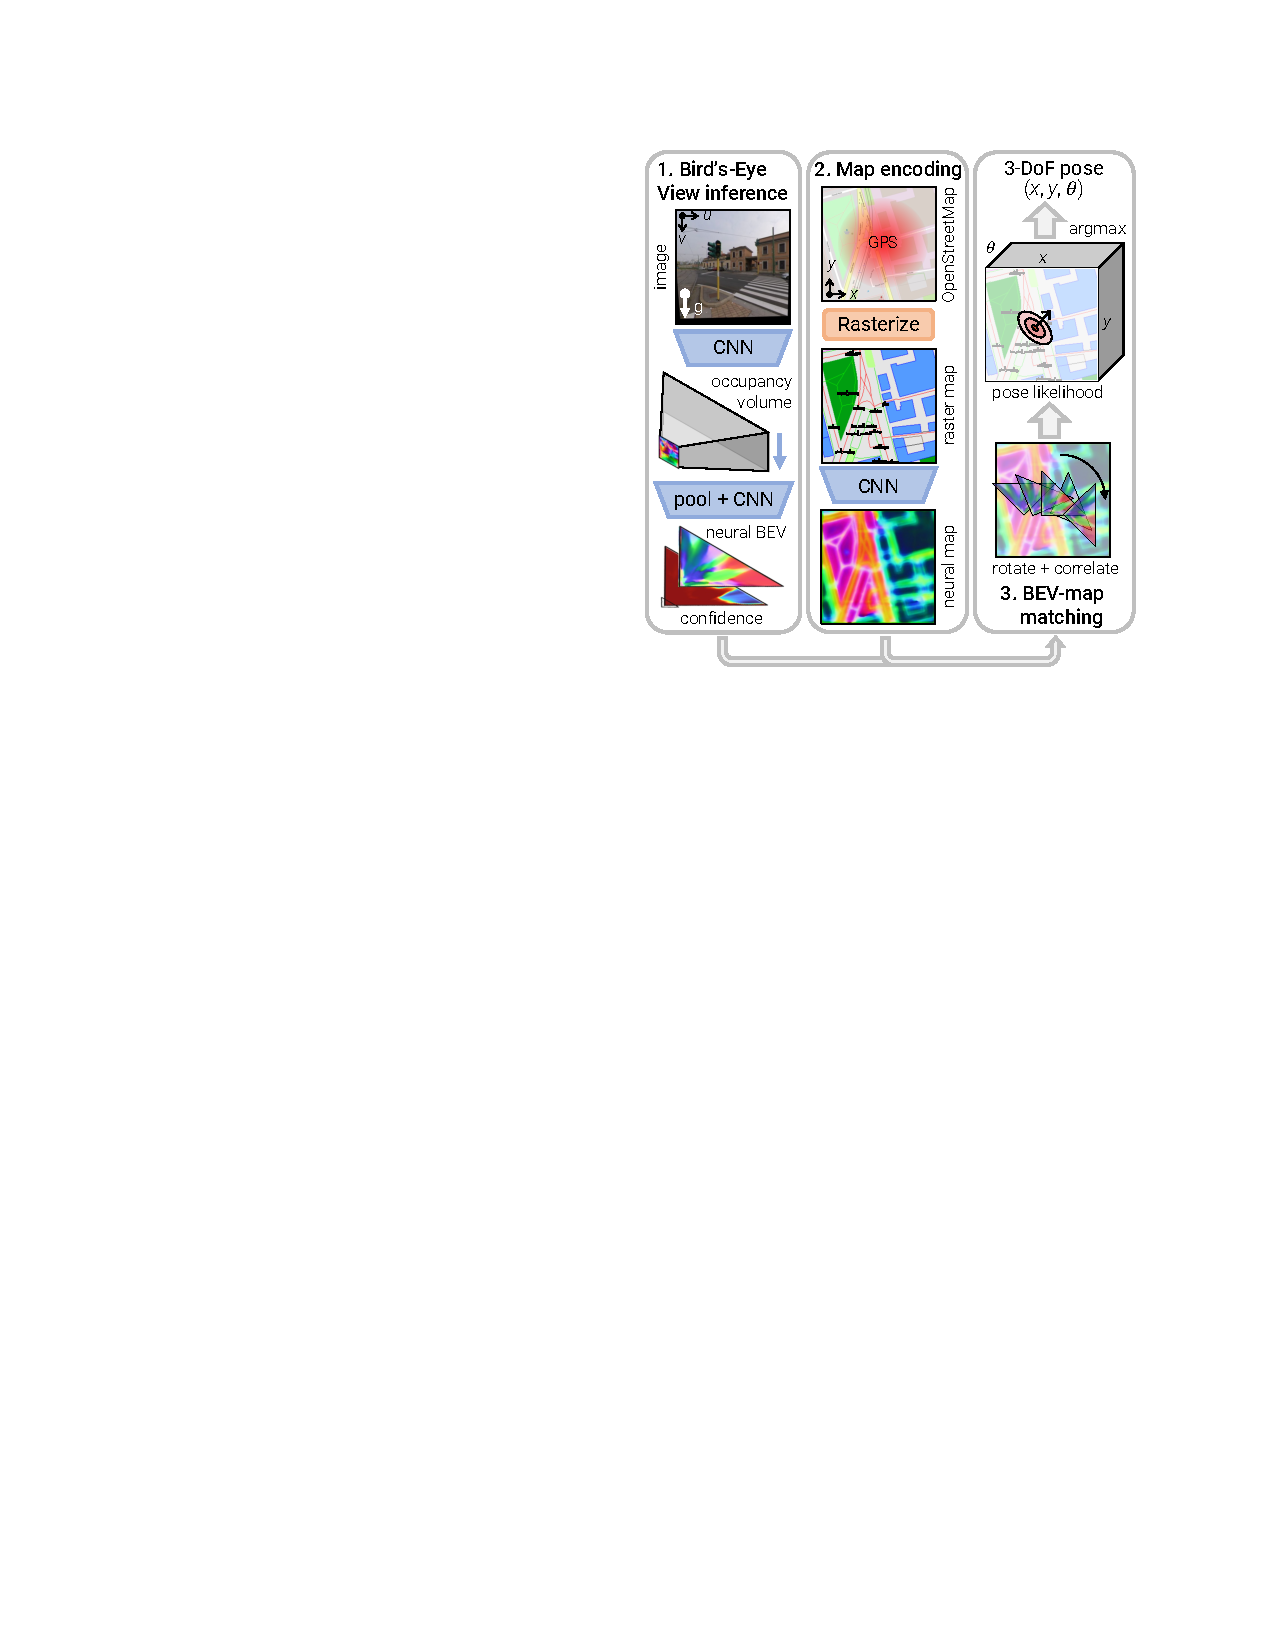
\includegraphics[width=0.55\linewidth]{LateX//figs/2304.02009v1.pdf}
    \caption{OrienterNet processes an input image \( I \) to generate a neural Bird’s-Eye View (BEV) \( T \) with associated confidence \( C \). Using a rough GPS location \( \boldsymbol{\xi}_{\text{prior}} \), a corresponding map is queried from OpenStreetMap. The BEV is then matched against the map \cite{sarlin2023orienternetvisuallocalization2d}.}
    \label{fig:orienternet}
\end{figure}


\begin{enumerate}
    \item \textit{Image-CNN}: Extracts semantic features from the input image \( I \) and projects them into an orthographic Bird’s-Eye View (BEV) representation \( T \) by inferring the 3D structure of the scene;
    \item \textit{Map-CNN}: Encodes the OSM map data into a neural map \( F \), embedding both semantic and geometric information;
    \item \textit{Pose Estimation}: Computes a probability distribution over camera poses \( \boldsymbol{\xi} \) by matching the BEV representation \( T \) against the map \( F \). 
\end{enumerate}

Another approach is presented in \textit{Visual Cross-View Metric Localization with Dense Uncertainty Estimates} \cite{xia2022visualcrossviewmetriclocalization}. The goal is to determine the location of a ground-level camera within a satellite image patch that shows the surrounding area. Unlike previous work that focused on range sensors (e.g., LiDAR, Radar) or used vision as a secondary regression step after cross-view image retrieval, this method focuses directly on metric localization. 

The implementation relies on the availability of a rough localization prior, which can be obtained from GPS/GNSS, Visual Odometry, or other robot localization techniques. As illustrated in Figure~\ref{fig:visual_cross_metric_architecture}, the architecture processes two input images: a ground-level image \( G \) and a top-down satellite image \( S \), both of size \( L \times L \), representing the local area where \( G \) was captured. The objective of the network is to estimate the 2D image coordinates \( X \in [0, 1]^2 \) within \( S \) that correspond to the ground camera's location. 
\begin{figure}[H]
    \centering
    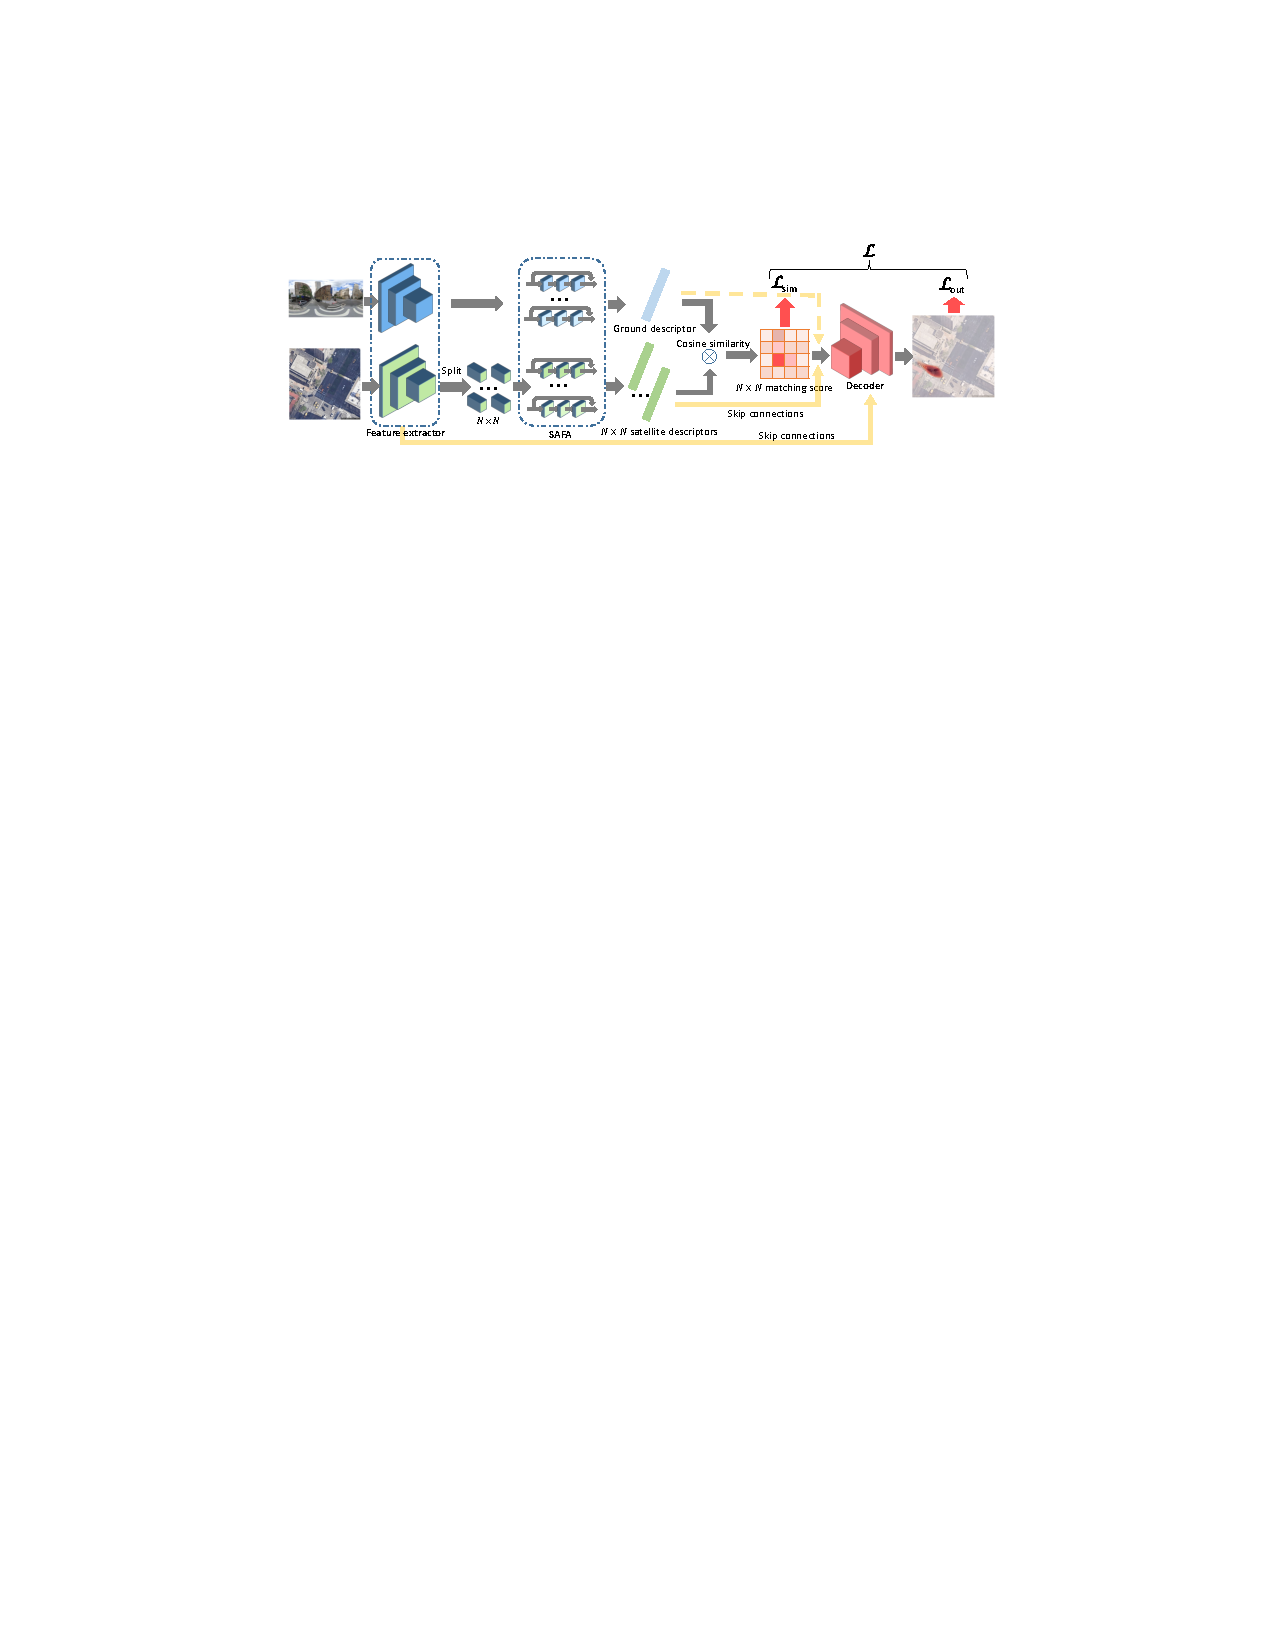
\includegraphics[width=1\linewidth]{LateX//figs/2208.08519v1.pdf}
    \caption{Network architecture for visual cross-view metric localization. The model takes a ground-level image \( G \) and a satellite image \( S \) as inputs and predicts the ground camera's location coordinates \( X \) \cite{xia2022visualcrossviewmetriclocalization}.}
    \label{fig:visual_cross_metric_architecture}
\end{figure}

The network uses a two-branch design where each input, like a ground-level or satellite image, is processed separately through a backbone to extract important features. In one branch, the features are adjusted into a fixed-size format for further processing. Spatial-aware modules are used to combine these features into smaller and more focused representations. The feature outputs from both branches are then joined together to create a single global descriptor.

The final related work discussed is \textit{BEV-Locator: An End-to-End Visual Semantic Localization Network Using Multi-View Images} \cite{zhang2022bevlocatorendtoendvisualsemantic}. It has been seen that traditional visual localization methods solve the semantic map-matching problem using geometric models. These models often require complex parameter tuning, which limits the scalability for large-scale applications. 

BEV-Locator, instead, introduces a different approach by using a neural network for end-to-end visual semantic localization with multi-view camera images. The system works as follows: A visual Bird’s-Eye-View (BEV) encoder processes and transforms multi-view images into the BEV space. Semantic map features are then encoded into structured vectors called map queries. A cross-modal transformer then associates BEV features with these map queries using cross-attention. At the end, by decoding the transformer's output, the ego vehicle's pose is estimated. 

The implementation, represented in Figure ~\ref{fig:bev-locator} includes:
\begin{figure}[H]
    \centering
    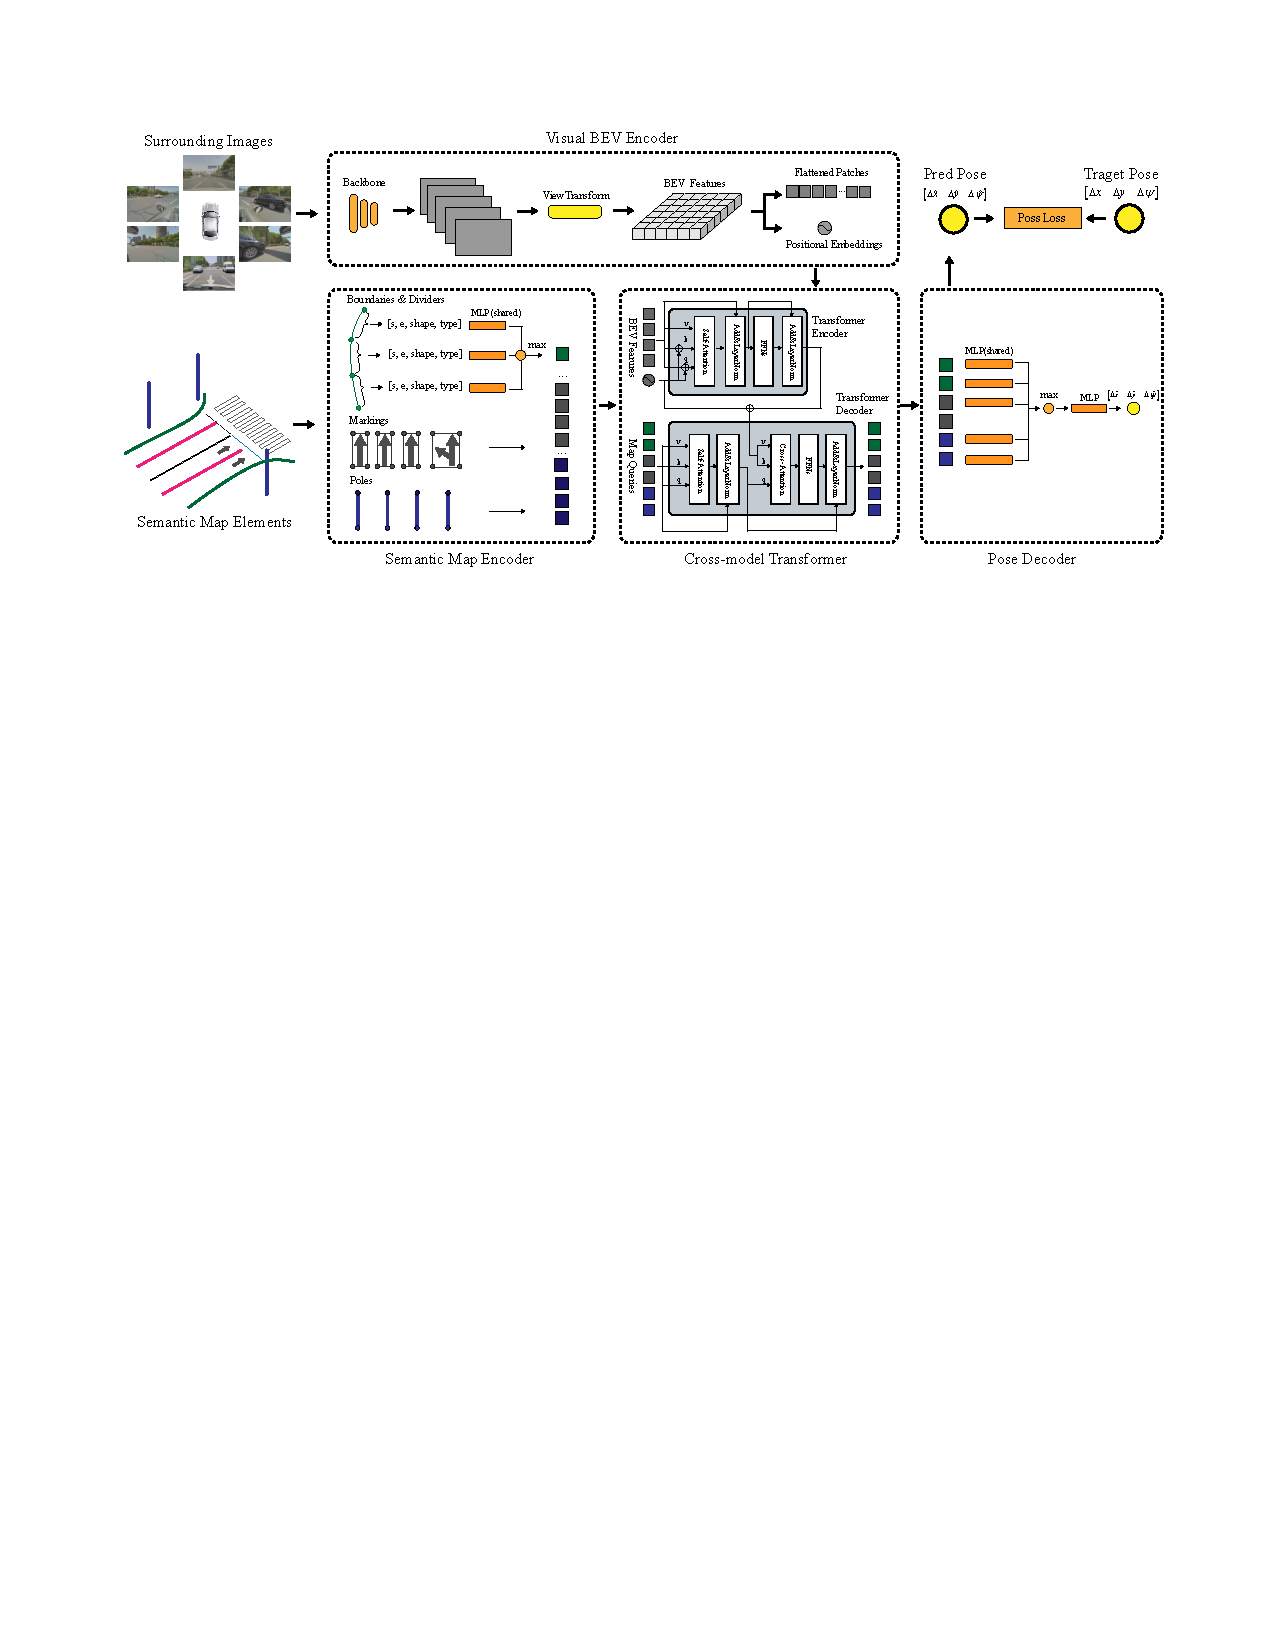
\includegraphics[width=1\linewidth]{LateX//figs/bevlocator.pdf}
    \caption{Overview of the system architecture, including the BEV Encoder, Semantic Map Encoder, Cross-Modal Transformer Module, and Pose Decoder \cite{zhang2022bevlocatorendtoendvisualsemantic}.}
    \label{fig:bev-locator}
\end{figure}

\begin{itemize}
    \item \textit{BEV Encoder:} Extracts features from surrounding images and projects them into BEV space;
    \item \textit{Semantic Map Encoder:} Encodes semantic map information into structural vectors, used as map queries for the transformer module;
    \item \textit{Cross-Modal Transformer:} Computes attention and queries the ego vehicle's pose using map queries and BEV features;
    \item \textit{Pose Decoder:} Converts the query vectors into the vehicle's pose.
\end{itemize}

MapAlign presents offline methods for localization on HD maps using deep learning-based neural networks to create ground truth automatically, inspired by the current State of the Art. Table~\ref{table:map_matching_methods} summarizes methods from neural networks, geometrical approaches, and other techniques. The results of these methods will be used for comparison in later sections.
\begin{table}[H]
\centering
\scriptsize
\caption{List of Map Matching Localization Methods \cite{Liu_Wang_Zhang_2020}.} 
\label{table:map_matching_methods}
\begin{tabular}{@{}
    >{\centering\arraybackslash}m{2.8cm}
    >{\centering\arraybackslash}m{0.6cm}
    >{\centering\arraybackslash}m{1.75cm}
    >{\centering\arraybackslash}m{2.2cm}
    >{\centering\arraybackslash}m{0.90cm}
    >{\centering\arraybackslash}m{0.95cm}
    >{\centering\arraybackslash}m{2.0cm}
    >{\centering\arraybackslash}m{0.75cm}
@{}}
\toprule
\textbf{Method} & \textbf{Year} & \textbf{Type} & \textbf{Map Types} & \textbf{Online} & \textbf{Offline} & \textbf{Sensors} & \textbf{Acc.} \\ 
\midrule
Points matching \cite{bernstein1996mapmatching} & 1996 & Geometric & Navigation map &  & \checkmark & GNSS & n/a \\
Arcs matching \cite{WHITE200091} & 2000 & Geometric & Navigation map & & \checkmark & GNSS & n/a \\
Frèchet Distance \cite{chen2011frechet} & 2011 & Geometric & Navigation map & & \checkmark & GNSS & n/a \\
Lane matching \cite{6629509} & 2013 & Feature matching & Vector map & \checkmark & & GNSS, IMU, Stereo & n/a \\
High Precision Maps \cite{6615239} & 2013 & Feature matching & Vector map & & \checkmark & GNSS, IMU, Monocular, LIDAR & 1.00 \\
Point Cloud matching \cite{6942558} & 2014 & Feature matching & Dense point cloud map &  & \checkmark & GNSS, IMU, Monocular, LIDAR & 0.25 \\
Road segment connectivity \cite{QUDDUS2015328} & 2015 & Geometric & Navigation map & & \checkmark & & n/a \\
Camera matching \cite{7759304} & 2016 & Feature matching & Dense point cloud map & & \checkmark & GNSS, Monocular & 0.30 \\
Point Group Association \cite{7528079} & 2016 & Landmark matching & Navigation map & & \checkmark & GNSS, MMW & n/a \\
Sensors Fusion \cite{7547970} & 2017 & Feature matching & Vector map & \checkmark & & GNSS, IMU, Monocular, Wheel encoder & 0.73 \\
HD Maps and GNSS \cite{li2017hdmaps} & 2017 & Particle filter & Navigation map & & \checkmark & GNSS, MMW & 4.70 \\
Fusion Map \cite{8317804} & 2018 & Multi hypotheses & Navigation map & & \checkmark & GNSS & 1.75 \\
Lane Marking matching \cite{8569951} & 2018 & Feature matching & Vector map & \checkmark & & LIDAR, GNSS, IMU & 0.04 \\
Visual Localization \cite{DBLP:journals/corr/abs-1801-05269} & 2018 & Feature matching & Dense point cloud map & & \checkmark & GNSS, Stereo & 0.60 \\
Compact Semantic Map \cite{DBLP:journals/corr/abs-1805-06155} & 2018 & Feature matching & Vector map & & \checkmark & IMU & 0.35 \\
Sparse Semantic Map \cite{DBLP:journals/corr/abs-1908-03274} & 2019 & Feature matching & Lightweight vector map &  & \checkmark & GNSS, IMU, Monocular & 0.51 \\
Closest Point (ICP) \cite{s20082166} & 2020 & Feature matching & Vector map & \checkmark & \checkmark & GNSS, IMU, Stereo, Mono, LIDAR & 0.48 \\
Monocular Localization \cite{s20071870} & 2020 & Feature matching & Lightweight vector map &  & \checkmark & GNSS, IMU, Monocular & 0.24 \\
VO and HD Maps \cite{9304659} & 2020 & Feature matching & Lightweight vector map & & \checkmark & GNSS, IMU, Stereo & 0.15 \\
Semantic Localization \cite{wang2021visual} & 2021 & Feature matching & Lightweight vector map & \checkmark & \checkmark & GNSS, Monocular, Wheel encoder & 0.13 \\
Microphones \cite{article11} & 2021 & Probabilistic model & Lightweight vector map & &\checkmark & GNSS, Microphone & 0.30 \\
Multi-sensors localization \cite{9772400} & 2022 & Neural network & Lightweight vector map & \checkmark & & GNSS, IMU, Monocular, Wheel encoder & 0.13 \\
Multi-view images \cite{zhang2022bevlocatorendtoendvisualsemantic} & 2022 & End-to-end learning & Lightweight vector map & \checkmark & & GNSS, IMU, Multi-view camera & 0.09 \\
Road shape matching \cite{article122} & 2023 & Geometric & Lightweight vector map & \checkmark & & GNSS, IMU, Monocular & 3.69 \\ \bottomrule
\end{tabular}
\end{table}